\documentclass[ngerman,a4paper,]{scrartcl}
\usepackage{lmodern}
\usepackage{amssymb,amsmath}
\usepackage{ifxetex,ifluatex}
\usepackage{fixltx2e} % provides \textsubscript
\ifnum 0\ifxetex 1\fi\ifluatex 1\fi=0 % if pdftex
  \usepackage[T1]{fontenc}
  \usepackage[utf8]{inputenc}
\else % if luatex or xelatex
  \ifxetex
    \usepackage{mathspec}
  \else
    \usepackage{fontspec}
  \fi
  \defaultfontfeatures{Ligatures=TeX,Scale=MatchLowercase}
    \setmainfont[]{TeX Gyre Pagella}
    \setsansfont[]{TeX Gyre Heros}
    \setmonofont[Mapping=tex-ansi,Mapping=tex-ansi,Scale=0.8]{Fira Mono}
    \setmathfont(Digits,Latin,Greek)[]{Asana Math}
\fi
% use upquote if available, for straight quotes in verbatim environments
\IfFileExists{upquote.sty}{\usepackage{upquote}}{}
% use microtype if available
\IfFileExists{microtype.sty}{%
\usepackage{microtype}
\UseMicrotypeSet[protrusion]{basicmath} % disable protrusion for tt fonts
}{}
\usepackage{hyperref}
\PassOptionsToPackage{usenames,dvipsnames}{color} % color is loaded by hyperref
\hypersetup{unicode=true,
            pdftitle={Poisson-Regression und ihre Leiden},
            pdfauthor={Lukas Burk},
            colorlinks=true,
            linkcolor=Maroon,
            citecolor=Blue,
            urlcolor=Blue,
            breaklinks=true}
\urlstyle{same}  % don't use monospace font for urls
\ifnum 0\ifxetex 1\fi\ifluatex 1\fi=0 % if pdftex
  \usepackage[shorthands=off,main=ngerman]{babel}
\else
  \usepackage{polyglossia}
  \setmainlanguage[]{german}
\fi
\usepackage{natbib}
\bibliographystyle{apalike}
\usepackage{color}
\usepackage{fancyvrb}
\newcommand{\VerbBar}{|}
\newcommand{\VERB}{\Verb[commandchars=\\\{\}]}
\DefineVerbatimEnvironment{Highlighting}{Verbatim}{commandchars=\\\{\}}
% Add ',fontsize=\small' for more characters per line
\usepackage{framed}
\definecolor{shadecolor}{RGB}{248,248,248}
\newenvironment{Shaded}{\begin{snugshade}}{\end{snugshade}}
\newcommand{\AlertTok}[1]{\textcolor[rgb]{0.94,0.16,0.16}{#1}}
\newcommand{\AnnotationTok}[1]{\textcolor[rgb]{0.56,0.35,0.01}{\textbf{\textit{#1}}}}
\newcommand{\AttributeTok}[1]{\textcolor[rgb]{0.77,0.63,0.00}{#1}}
\newcommand{\BaseNTok}[1]{\textcolor[rgb]{0.00,0.00,0.81}{#1}}
\newcommand{\BuiltInTok}[1]{#1}
\newcommand{\CharTok}[1]{\textcolor[rgb]{0.31,0.60,0.02}{#1}}
\newcommand{\CommentTok}[1]{\textcolor[rgb]{0.56,0.35,0.01}{\textit{#1}}}
\newcommand{\CommentVarTok}[1]{\textcolor[rgb]{0.56,0.35,0.01}{\textbf{\textit{#1}}}}
\newcommand{\ConstantTok}[1]{\textcolor[rgb]{0.00,0.00,0.00}{#1}}
\newcommand{\ControlFlowTok}[1]{\textcolor[rgb]{0.13,0.29,0.53}{\textbf{#1}}}
\newcommand{\DataTypeTok}[1]{\textcolor[rgb]{0.13,0.29,0.53}{#1}}
\newcommand{\DecValTok}[1]{\textcolor[rgb]{0.00,0.00,0.81}{#1}}
\newcommand{\DocumentationTok}[1]{\textcolor[rgb]{0.56,0.35,0.01}{\textbf{\textit{#1}}}}
\newcommand{\ErrorTok}[1]{\textcolor[rgb]{0.64,0.00,0.00}{\textbf{#1}}}
\newcommand{\ExtensionTok}[1]{#1}
\newcommand{\FloatTok}[1]{\textcolor[rgb]{0.00,0.00,0.81}{#1}}
\newcommand{\FunctionTok}[1]{\textcolor[rgb]{0.00,0.00,0.00}{#1}}
\newcommand{\ImportTok}[1]{#1}
\newcommand{\InformationTok}[1]{\textcolor[rgb]{0.56,0.35,0.01}{\textbf{\textit{#1}}}}
\newcommand{\KeywordTok}[1]{\textcolor[rgb]{0.13,0.29,0.53}{\textbf{#1}}}
\newcommand{\NormalTok}[1]{#1}
\newcommand{\OperatorTok}[1]{\textcolor[rgb]{0.81,0.36,0.00}{\textbf{#1}}}
\newcommand{\OtherTok}[1]{\textcolor[rgb]{0.56,0.35,0.01}{#1}}
\newcommand{\PreprocessorTok}[1]{\textcolor[rgb]{0.56,0.35,0.01}{\textit{#1}}}
\newcommand{\RegionMarkerTok}[1]{#1}
\newcommand{\SpecialCharTok}[1]{\textcolor[rgb]{0.00,0.00,0.00}{#1}}
\newcommand{\SpecialStringTok}[1]{\textcolor[rgb]{0.31,0.60,0.02}{#1}}
\newcommand{\StringTok}[1]{\textcolor[rgb]{0.31,0.60,0.02}{#1}}
\newcommand{\VariableTok}[1]{\textcolor[rgb]{0.00,0.00,0.00}{#1}}
\newcommand{\VerbatimStringTok}[1]{\textcolor[rgb]{0.31,0.60,0.02}{#1}}
\newcommand{\WarningTok}[1]{\textcolor[rgb]{0.56,0.35,0.01}{\textbf{\textit{#1}}}}
\usepackage{longtable,booktabs}
\usepackage{graphicx,grffile}
\makeatletter
\def\maxwidth{\ifdim\Gin@nat@width>\linewidth\linewidth\else\Gin@nat@width\fi}
\def\maxheight{\ifdim\Gin@nat@height>\textheight\textheight\else\Gin@nat@height\fi}
\makeatother
% Scale images if necessary, so that they will not overflow the page
% margins by default, and it is still possible to overwrite the defaults
% using explicit options in \includegraphics[width, height, ...]{}
\setkeys{Gin}{width=\maxwidth,height=\maxheight,keepaspectratio}
% Make links footnotes instead of hotlinks:
\renewcommand{\href}[2]{#2\footnote{\url{#1}}}
\IfFileExists{parskip.sty}{%
\usepackage{parskip}
}{% else
\setlength{\parindent}{0pt}
\setlength{\parskip}{6pt plus 2pt minus 1pt}
}
\setlength{\emergencystretch}{3em}  % prevent overfull lines
\providecommand{\tightlist}{%
  \setlength{\itemsep}{0pt}\setlength{\parskip}{0pt}}
\setcounter{secnumdepth}{5}
% Redefines (sub)paragraphs to behave more like sections
\ifx\paragraph\undefined\else
\let\oldparagraph\paragraph
\renewcommand{\paragraph}[1]{\oldparagraph{#1}\mbox{}}
\fi
\ifx\subparagraph\undefined\else
\let\oldsubparagraph\subparagraph
\renewcommand{\subparagraph}[1]{\oldsubparagraph{#1}\mbox{}}
\fi

%%% Use protect on footnotes to avoid problems with footnotes in titles
\let\rmarkdownfootnote\footnote%
\def\footnote{\protect\rmarkdownfootnote}

%%% Change title format to be more compact
\usepackage{titling}

% Create subtitle command for use in maketitle
\providecommand{\subtitle}[1]{
  \posttitle{
    \begin{center}\large#1\end{center}
    }
}

\setlength{\droptitle}{-2em}

  \title{Poisson-Regression und ihre Leiden}
    \pretitle{\vspace{\droptitle}\centering\huge}
  \posttitle{\par}
    \author{Lukas Burk}
    \preauthor{\centering\large\emph}
  \postauthor{\par}
      \predate{\centering\large\emph}
  \postdate{\par}
    \date{Stand: 11. September 2019 10:57 Uhr (CEST)}

\usepackage{booktabs}
\usepackage{longtable}
\usepackage{float}
\usepackage{csquotes}
\usepackage{tabularx}
\usepackage{tabu}
\usepackage{array}
\usepackage{multirow}
\usepackage{wrapfig}

% unicode-math seems to be the preferred superset of mathspec (and fontspec?)
% ISO means bold math is set italics, =TeX would make bold math upright
%\usepackage[bold-style=ISO]{unicode-math}

%\urlstyle{tt}
\usepackage{booktabs}
\usepackage{longtable}
\usepackage{array}
\usepackage{multirow}
\usepackage{wrapfig}
\usepackage{float}
\usepackage{colortbl}
\usepackage{pdflscape}
\usepackage{tabu}
\usepackage{threeparttable}
\usepackage{threeparttablex}
\usepackage[normalem]{ulem}
\usepackage{makecell}
\usepackage{xcolor}

\usepackage{amsthm}
\newtheorem{theorem}{Theorem}[section]
\newtheorem{lemma}{Lemma}[section]
\newtheorem{corollary}{Corollary}[section]
\newtheorem{proposition}{Proposition}[section]
\newtheorem{conjecture}{Conjecture}[section]
\theoremstyle{definition}
\newtheorem{definition}{Definition}[section]
\theoremstyle{definition}
\newtheorem{example}{Example}[section]
\theoremstyle{definition}
\newtheorem{exercise}{Exercise}[section]
\theoremstyle{remark}
\newtheorem*{remark}{Remark}
\newtheorem*{solution}{Solution}
\let\BeginKnitrBlock\begin \let\EndKnitrBlock\end
\begin{document}
\maketitle

{
\hypersetup{linkcolor=black}
\setcounter{tocdepth}{2}
\tableofcontents
}
\hypertarget{einfuhrung}{%
\section{Einführung}\label{einfuhrung}}

Dieses Dokument soll einen Überblick zum Umgang mit Zähldaten (\emph{count data}) liefern.\\
Zähldaten können im Allgemeinen mittels Poissonverteilung im Rahmen des GLM modelliert werden, allerdings sind in der Praxis einige Komplikationen zu erwarten:

\textbf{Over-/underdispersion} (siehe Abschnitt \ref{dispersion}): Die Poissonverteilung besitzt nur einen Parameter für sowohl Erwartungswert als auch Varianz und nimmt somit Gleichheit zwischen den beiden an (\emph{equidispersion}) -- diese Annahme ist meist in Form von overdispersion verletzt

\textbf{Zero-Inflation} (siehe Abschnitt \ref{zeros}): Aus einem Modell lässt sich die erwartete Anzahl an Beobachtungen mit Anzahl \(0\) bestimmen -- wenn die beobachtete Anzahl (bzw. der Anteil) an Nullen deutlich größer ist, spricht man von \emph{zero-inflation}. Verwandte Probleme sind die (seltenere) \emph{zero-deflation}, oder das strukturelle Fehlen von Nullen

Diese Umstände benötigen in der Regel Generalisierungen der einfach Poisson-Regression, entweder durch Erweiterung der Verteilung um zusätzliche Parameter (siehe z.B. \emph{Negative Binomialverteilung} für overdispersion in Abschnitt \ref{mod-nb}, \emph{Generalized Poisson} für underdispersion in Abschnitt \ref{mod-gp}) oder die Konstruktion von \emph{mixture models} oder \emph{hurdle models} für zero-inflation (Abschnitte \ref{mod-zi} und \ref{mod-hurdle}).

\hypertarget{data}{%
\subsection{Beispieldaten}\label{data}}

Als Anwendungsbeispiele werden einige Datensätze verwendet, die verschiedene Probleme illustrieren:

\begin{itemize}
\tightlist
\item
  \texttt{azprocedure}: Patienten kardiovaskulärer Behandlungen in Arizona

  \begin{itemize}
  \tightlist
  \item
    Count: \texttt{los}, Dauer eines Krankenhausaufenthalts in Tagen (1 - 83)
  \item
    Kovariablen:

    \begin{itemize}
    \tightlist
    \item
      \texttt{sex}: Male (1), female(0)
    \item
      \texttt{admit}: Type of admission. Urgent/emergency (1), elective (0)
    \end{itemize}
  \end{itemize}
\item
  \texttt{rwm5yr} (\texttt{rwm1984}): \enquote{German health registry} 1984-1988 (bzw. nur 1984)

  \begin{itemize}
  \tightlist
  \item
    Count: \texttt{docvis}: Anzahl der Arztbesuche (0 - 121)
  \item
    Kovariablen:

    \begin{itemize}
    \tightlist
    \item
      \texttt{outwork}: Arbeitslos (1), arbeitend (0)
    \item
      \texttt{age}: Alter (25 - 64)
    \end{itemize}
  \end{itemize}
\item
  \texttt{fish}: Geangelte Fische an einem Campingwochenende

  \begin{itemize}
  \tightlist
  \item
    Count: \texttt{count}, Anzahl der Fische
  \item
    Kovariablen:

    \begin{itemize}
    \tightlist
    \item
      \texttt{child}: Anzahl der Kinder in der Campergruppe
    \item
      \texttt{persons}: Anzahl der Personen in der Campergruppe
    \item
      \texttt{camper}: \texttt{{[}0,\ 1{]}} Hat die Gruppe einen Campingwagen mitgebracht?
    \end{itemize}
  \end{itemize}
\end{itemize}

Diese Datensätze finden sich entweder in R-packages oder auf der website der UCLA IDRE:

\begin{table}[H]
\centering
\begin{tabular}{lll}
\toprule
Dataset & R Package & Quelle\\
\midrule
azprocedure & COUNT & Hilbe (2014)\\
rwm5yr & COUNT & Hilbe (2014)\\
rwm1984 & COUNT & Hilbe (2014)\\
nuts & COUNT & Hilbe (2014)\\
fish & – & UCLA IDRE (https://stats.idre.ucla.edu)\\
\bottomrule
\end{tabular}
\end{table}

Daten aus \citet{hilbeModelingCountData2014} sind zusätzlich verfügbar als CSV (\texttt{HILBE-MCD-CVS-data}) auf \href{https://works.bepress.com/joseph_hilbe/58/}{der Website des Autors}.

Die Datensätze des UCLA IDRE können wie folgt eingelesen werden:

\begin{Shaded}
\begin{Highlighting}[]
\NormalTok{fish <-}\StringTok{ }\NormalTok{haven}\OperatorTok{::}\KeywordTok{read_sas}\NormalTok{(}\StringTok{"https://stats.idre.ucla.edu/stat/sas/code/fish.sas7bdat"}\NormalTok{)}

\CommentTok{# Cache locally}
\KeywordTok{saveRDS}\NormalTok{(fish, }\StringTok{"data/fish.rds"}\NormalTok{)}

\CommentTok{# Read from cache later:}
\CommentTok{# fish <- readRDS("data/fish.rds")}
\end{Highlighting}
\end{Shaded}

Um Daten aus \texttt{R} direkt in SAS-freundlichem \texttt{sas7bdat} zu speichern, kann folgender Code unter Verwendung des packages \href{https://haven.tidyverse.org/}{\texttt{haven}} verwendet werden:

\begin{Shaded}
\begin{Highlighting}[]
\CommentTok{# Install package 'haven' if required}
\ControlFlowTok{if}\NormalTok{ (}\OperatorTok{!}\NormalTok{(}\StringTok{"haven"} \OperatorTok\StringTok{ }\KeywordTok{installed.packages}\NormalTok{())) \{}
   \KeywordTok{install.packages}\NormalTok{(}\StringTok{"haven"}\NormalTok{)}
\NormalTok{\}}
\CommentTok{# Load some example data}
\KeywordTok{data}\NormalTok{(}\StringTok{"azprocedure"}\NormalTok{, }\DataTypeTok{package =} \StringTok{"COUNT"}\NormalTok{)}
\CommentTok{# Write in SAS-format}
\NormalTok{haven}\OperatorTok{::}\KeywordTok{write_sas}\NormalTok{(azprocedure, }\StringTok{"path/to/saved/file.sas7bdat"}\NormalTok{)}
\end{Highlighting}
\end{Shaded}

\hypertarget{software-funs}{%
\subsection{Verwendete Software}\label{software-funs}}

Um Code-Beispiele (und Output) übersichtlich zu halten werden einige R-Packages und Hilfsfunktionen verwendet, die hier kurz beschrieben werden um Code in späteren Abschnitten nachvollziehbar zu halten.\\
Siehe dazu auch Anhang \ref{repro}.

\hypertarget{r-packages}{%
\subsubsection{R-Packages}\label{r-packages}}

Zur Reproduktion der Beispiele sind insbesondere die folgenden \texttt{R} packages notwendig, die durch den angegebenen Code installiert werden, sofern sie nicht bereits verfügbar sind:

\begin{Shaded}
\begin{Highlighting}[]
\CommentTok{# Data transformation / modelling}
\ControlFlowTok{if}\NormalTok{ (}\OperatorTok{!}\NormalTok{(}\StringTok{"dplyr"} \OperatorTok\StringTok{ }\KeywordTok{installed.packages}\NormalTok{())) }\KeywordTok{install.packages}\NormalTok{(}\StringTok{"dplyr"}\NormalTok{)}
\ControlFlowTok{if}\NormalTok{ (}\OperatorTok{!}\NormalTok{(}\StringTok{"purrr"} \OperatorTok\StringTok{ }\KeywordTok{installed.packages}\NormalTok{())) }\KeywordTok{install.packages}\NormalTok{(}\StringTok{"purrr"}\NormalTok{)}
\ControlFlowTok{if}\NormalTok{ (}\OperatorTok{!}\NormalTok{(}\StringTok{"broom"} \OperatorTok\StringTok{ }\KeywordTok{installed.packages}\NormalTok{())) }\KeywordTok{install.packages}\NormalTok{(}\StringTok{"broom"}\NormalTok{)}

\CommentTok{# Plots}
\ControlFlowTok{if}\NormalTok{ (}\OperatorTok{!}\NormalTok{(}\StringTok{"ggplot2"} \OperatorTok\StringTok{ }\KeywordTok{installed.packages}\NormalTok{())) }\KeywordTok{install.packages}\NormalTok{(}\StringTok{"ggplot2"}\NormalTok{)}

\CommentTok{# Modelling}
\ControlFlowTok{if}\NormalTok{ (}\OperatorTok{!}\NormalTok{(}\StringTok{"lmtest"} \OperatorTok\StringTok{ }\KeywordTok{installed.packages}\NormalTok{())) }\KeywordTok{install.packages}\NormalTok{(}\StringTok{"lmtest"}\NormalTok{)}
\ControlFlowTok{if}\NormalTok{ (}\OperatorTok{!}\NormalTok{(}\StringTok{"msme"} \OperatorTok\StringTok{ }\KeywordTok{installed.packages}\NormalTok{())) }\KeywordTok{install.packages}\NormalTok{(}\StringTok{"msme"}\NormalTok{)}
\ControlFlowTok{if}\NormalTok{ (}\OperatorTok{!}\NormalTok{(}\StringTok{"VGAM"} \OperatorTok\StringTok{ }\KeywordTok{installed.packages}\NormalTok{())) }\KeywordTok{install.packages}\NormalTok{(}\StringTok{"VGAM"}\NormalTok{)}
\ControlFlowTok{if}\NormalTok{ (}\OperatorTok{!}\NormalTok{(}\StringTok{"gamlss"} \OperatorTok\StringTok{ }\KeywordTok{installed.packages}\NormalTok{())) }\KeywordTok{install.packages}\NormalTok{(}\StringTok{"gamlss"}\NormalTok{)}

\CommentTok{# Data (and maybe modelling)}
\ControlFlowTok{if}\NormalTok{ (}\OperatorTok{!}\NormalTok{(}\StringTok{"COUNT"} \OperatorTok\StringTok{ }\KeywordTok{installed.packages}\NormalTok{())) }\KeywordTok{install.packages}\NormalTok{(}\StringTok{"COUNT"}\NormalTok{)}

\CommentTok{# Output formatting (for RMarkdown/pandoc markdown documents)}
\ControlFlowTok{if}\NormalTok{ (}\OperatorTok{!}\NormalTok{(}\StringTok{"pander"} \OperatorTok\StringTok{ }\KeywordTok{installed.packages}\NormalTok{())) }\KeywordTok{install.packages}\NormalTok{(}\StringTok{"pander"}\NormalTok{)}
\ControlFlowTok{if}\NormalTok{ (}\OperatorTok{!}\NormalTok{(}\StringTok{"kableExtra"} \OperatorTok\StringTok{ }\KeywordTok{installed.packages}\NormalTok{())) }\KeywordTok{install.packages}\NormalTok{(}\StringTok{"kableExtra"}\NormalTok{)}
\end{Highlighting}
\end{Shaded}

Siehe auch Anhang \ref{repro} zu verwendeten Packages.

\hypertarget{helperfuns}{%
\subsubsection{Funktionen}\label{helperfuns}}

Weiterhin werden einige Hilfsfunktionen im Laufe des Dokuments verwendet, die primär der Abkürzung und/oder der Formatierung des Outputs dienen:

\begin{Shaded}
\begin{Highlighting}[]
\CommentTok{#' Simple descriptive stats for count variables}
\CommentTok{#' @param x A count variable, presumed to be a non-negative integer.}
\CommentTok{#' @param digits Number of digits to round statistics to.}
\CommentTok{#' @return Nichts, nur print output.}
\NormalTok{describe_counts <-}\StringTok{ }\ControlFlowTok{function}\NormalTok{(x, }\DataTypeTok{digits =} \DecValTok{2}\NormalTok{) \{}
   \KeywordTok{require}\NormalTok{(kableExtra)}
   
\NormalTok{   tibble}\OperatorTok{::}\KeywordTok{tibble}\NormalTok{(}
      \DataTypeTok{n =} \KeywordTok{length}\NormalTok{(x),}
      \DataTypeTok{missing =} \KeywordTok{sum}\NormalTok{(}\KeywordTok{is.na}\NormalTok{(x)),}
      \DataTypeTok{mean =} \KeywordTok{round}\NormalTok{(}\KeywordTok{mean}\NormalTok{(x, }\DataTypeTok{na.rm =} \OtherTok{TRUE}\NormalTok{), digits),}
      \DataTypeTok{var =} \KeywordTok{round}\NormalTok{(}\KeywordTok{var}\NormalTok{(x, }\DataTypeTok{na.rm =} \OtherTok{TRUE}\NormalTok{), digits),}
      \DataTypeTok{range =} \KeywordTok{paste0}\NormalTok{(}\StringTok{"["}\NormalTok{, }\KeywordTok{paste0}\NormalTok{(}\KeywordTok{range}\NormalTok{(x, }\DataTypeTok{na.rm =} \OtherTok{TRUE}\NormalTok{), }\DataTypeTok{collapse =} \StringTok{", "}\NormalTok{), }\StringTok{"]"}\NormalTok{)}
\NormalTok{   ) }\OperatorTok
\StringTok{   }\KeywordTok{setNames}\NormalTok{(}\KeywordTok{c}\NormalTok{(}\StringTok{"N"}\NormalTok{, }\StringTok{"Missing"}\NormalTok{, }\StringTok{"Mittelwert"}\NormalTok{, }\StringTok{"Varianz"}\NormalTok{, }\StringTok{"Range"}\NormalTok{)) }\OperatorTok
\StringTok{   }\KeywordTok{kable}\NormalTok{(}\DataTypeTok{booktabs =} \OtherTok{TRUE}\NormalTok{, }\DataTypeTok{escape =} \OtherTok{FALSE}\NormalTok{, }\DataTypeTok{linesep =} \StringTok{""}\NormalTok{) }\OperatorTok
\StringTok{   }\KeywordTok{kable_styling}\NormalTok{(}\DataTypeTok{position =} \StringTok{"center"}\NormalTok{, }\DataTypeTok{protect_latex =} \OtherTok{TRUE}\NormalTok{)}
\NormalTok{\}}
\CommentTok{# Example usage}
\CommentTok{# Define random count variable...}
\NormalTok{x <-}\StringTok{ }\KeywordTok{rpois}\NormalTok{(}\DecValTok{100}\NormalTok{, }\DecValTok{5}\NormalTok{)}

\CommentTok{# ...with some missings}
\NormalTok{x[}\KeywordTok{sample}\NormalTok{(}\DecValTok{100}\NormalTok{, }\DecValTok{10}\NormalTok{)] <-}\StringTok{ }\OtherTok{NA}

\CommentTok{# A basic summary}
\KeywordTok{describe_counts}\NormalTok{(x)}
\end{Highlighting}
\end{Shaded}

\begin{table}[H]
\centering
\begin{tabular}{rrrrl}
\toprule
N & Missing & Mittelwert & Varianz & Range\\
\midrule
100 & 10 & 5.06 & 5.51 & [1, 10]\\
\bottomrule
\end{tabular}
\end{table}

Die Pearson-Dispersionsstatistik (eingeführt in Abschnitt \ref{dispersion}, Definition \ref{def:def-pearsondisp}):

\begin{Shaded}
\begin{Highlighting}[]
\CommentTok{#' Pearson-Dispersion}
\CommentTok{#' @param model Ein `glm`-Objekt mit Methoden für `resid()` und `df.residual`-Komponente}
\CommentTok{#' @param type Entweder 'pearson' (default) oder 'deviance'.}
\CommentTok{#' @return Invisible: Liste mit chi^2-Statistik, Freiheitsgraden und Dispersion.}
\CommentTok{#'         Printed: Formatiertes output.}
\NormalTok{dispersion <-}\StringTok{ }\ControlFlowTok{function}\NormalTok{(model, }\DataTypeTok{type =} \StringTok{"pearson"}\NormalTok{) \{}
\NormalTok{  chisq <-}\StringTok{ }\KeywordTok{sum}\NormalTok{(}\KeywordTok{resid}\NormalTok{(model, }\DataTypeTok{type =}\NormalTok{ type)}\OperatorTok{^}\DecValTok{2}\NormalTok{)}
\NormalTok{  disp  <-}\StringTok{ }\NormalTok{chisq }\OperatorTok{/}\StringTok{ }\NormalTok{model}\OperatorTok{$}\NormalTok{df.residual}
  
  \KeywordTok{invisible}\NormalTok{(}\KeywordTok{list}\NormalTok{(}\DataTypeTok{chi2 =}\NormalTok{ chisq, }\DataTypeTok{df =}\NormalTok{ model}\OperatorTok{$}\NormalTok{df.residual, }\DataTypeTok{dispersion =}\NormalTok{ disp))}
  \KeywordTok{cat}\NormalTok{(}\KeywordTok{sprintf}\NormalTok{(}\StringTok{"X-squared(%i) = %.2f}\CharTok{\textbackslash{}n}\StringTok{%s Dispersion = %.3f"}\NormalTok{, model}\OperatorTok{$}\NormalTok{df.residual,  }
\NormalTok{              chisq, }\KeywordTok{chartr}\NormalTok{(}\StringTok{"pd"}\NormalTok{, }\StringTok{"PD"}\NormalTok{, type), disp))}
\NormalTok{\}}
\end{Highlighting}
\end{Shaded}

Der \emph{Lagrange Multiplier Test}:

\begin{Shaded}
\begin{Highlighting}[]
\CommentTok{#' Lagrange Multiplier Test according to Hilbe (2014)}
\CommentTok{#' @param model A `glm` or similiar object.}
\CommentTok{#' @return Chi^2 statistic and corresponding p-value in a list of class "htest".}
\NormalTok{lagrange_test <-}\StringTok{ }\ControlFlowTok{function}\NormalTok{(model) \{}
\NormalTok{   mu     <-}\StringTok{ }\KeywordTok{predict}\NormalTok{(model, }\DataTypeTok{type =} \StringTok{"response"}\NormalTok{)}
\NormalTok{   n_ybar <-}\StringTok{ }\KeywordTok{length}\NormalTok{(model}\OperatorTok{$}\NormalTok{y) }\OperatorTok{*}\StringTok{ }\KeywordTok{mean}\NormalTok{(mu)}
\NormalTok{   mu2    <-}\StringTok{ }\KeywordTok{mean}\NormalTok{(mu}\OperatorTok{^}\DecValTok{2}\NormalTok{) }\OperatorTok{*}\StringTok{ }\KeywordTok{length}\NormalTok{(model}\OperatorTok{$}\NormalTok{y)}
\NormalTok{   chisq  <-}\StringTok{ }\NormalTok{(mu2 }\OperatorTok{-}\StringTok{ }\NormalTok{n_ybar)}\OperatorTok{^}\DecValTok{2} \OperatorTok{/}\StringTok{ }\NormalTok{(}\DecValTok{2} \OperatorTok{*}\StringTok{ }\NormalTok{mu2)}
   \KeywordTok{names}\NormalTok{(chisq) <-}\StringTok{ "X-squared"}
\NormalTok{   pval   <-}\StringTok{ }\KeywordTok{pchisq}\NormalTok{(chisq, }\DataTypeTok{df =} \DecValTok{1}\NormalTok{, }\DataTypeTok{lower.tail =} \OtherTok{FALSE}\NormalTok{)}
\NormalTok{   df <-}\StringTok{ }\DecValTok{1}
   \KeywordTok{names}\NormalTok{(df) <-}\StringTok{ "df"}
  
\NormalTok{   rval <-}\StringTok{ }\KeywordTok{list}\NormalTok{(}
      \DataTypeTok{statistic =}\NormalTok{ chisq, }\DataTypeTok{parameter =}\NormalTok{ df, }\DataTypeTok{p.value =}\NormalTok{ pval,}
      \DataTypeTok{alternative =} \StringTok{"Data is overdispersed"}\NormalTok{, }
      \DataTypeTok{method =} \StringTok{"Lagrange Multiplier Test"}\NormalTok{, }
      \DataTypeTok{data.name =} \KeywordTok{deparse}\NormalTok{(mod}\OperatorTok{$}\NormalTok{call)}
\NormalTok{   )}
   
   \KeywordTok{class}\NormalTok{(rval) <-}\StringTok{ "htest"}
\NormalTok{   rval}
\NormalTok{\}}
\end{Highlighting}
\end{Shaded}

\hypertarget{poisson-modell}{%
\section{Das Poisson-Modell}\label{poisson-modell}}

Das Poisson-Modell ist die allgemeine Grundlage für die Modellierung von Zählvorgängen / Counts, und auch wenn es in seiner \enquote{reinen} Form in der Praxis meist nicht ausreicht, bauen alle weiteren Methoden auf die eine oder andere Art darauf auf. Auch die häufig verwendete Negative Binomialverteilung ist letztlich eine Poisson-Verteilung mit Gamma-verteilter Varianz, also eine Erweiterung der Poisson um einen zusätzlichen Parameter. Das gleiche Prinzip findet sich in allen hier besprochenen Verteilungen.

Für eine ausführliche Diskussion der Eigenschaften, siehe \citet{winkelmannEconometricAnalysisCount2010} (p.~7-20).

Grundlage zur Modellierung ist das GLM mit den dazugehörigen Voraussetzungen:

\begin{itemize}
\tightlist
\item
  Die abhängige Variable \(Y\) kommt aus der Exponentialfamilie (Normal-, Poisson-, Gamma-, Binomialverteilung)
\item
  Modelliert wird der lineare Prädiktor \(\eta_i = \boldsymbol{x}_i' \boldsymbol{\beta}\).
\item
  Response- und Linkfunktionen \(h(x)\) und \(g(x) = h^{-1}(x)\)
\end{itemize}

\BeginKnitrBlock{definition}[Poisson-Verteilung]
\protect\hypertarget{def:unnamed-chunk-1}{}{\label{def:unnamed-chunk-1} \iffalse (Poisson-Verteilung) \fi{} }Eine Poisson-verteilte Zufallsvariable \(Y \sim \mathrm{Poi}(\mu)\) \footnote{Der Poisson-Parameter wird von unterschiedlichen Autoren als \(\lambda\) oder \(\mu\) bezeichnet, und ich habe mich noch nicht für eine Variante entschieden).} hat die Dichte

\begin{equation*}
\mathrm{P}(Y = y) = \frac{\mu^y \exp(-\mu)}{y!} \quad, y \in \mathbb{N}_0
\end{equation*}
\EndKnitrBlock{definition}

\begin{figure}

{\centering 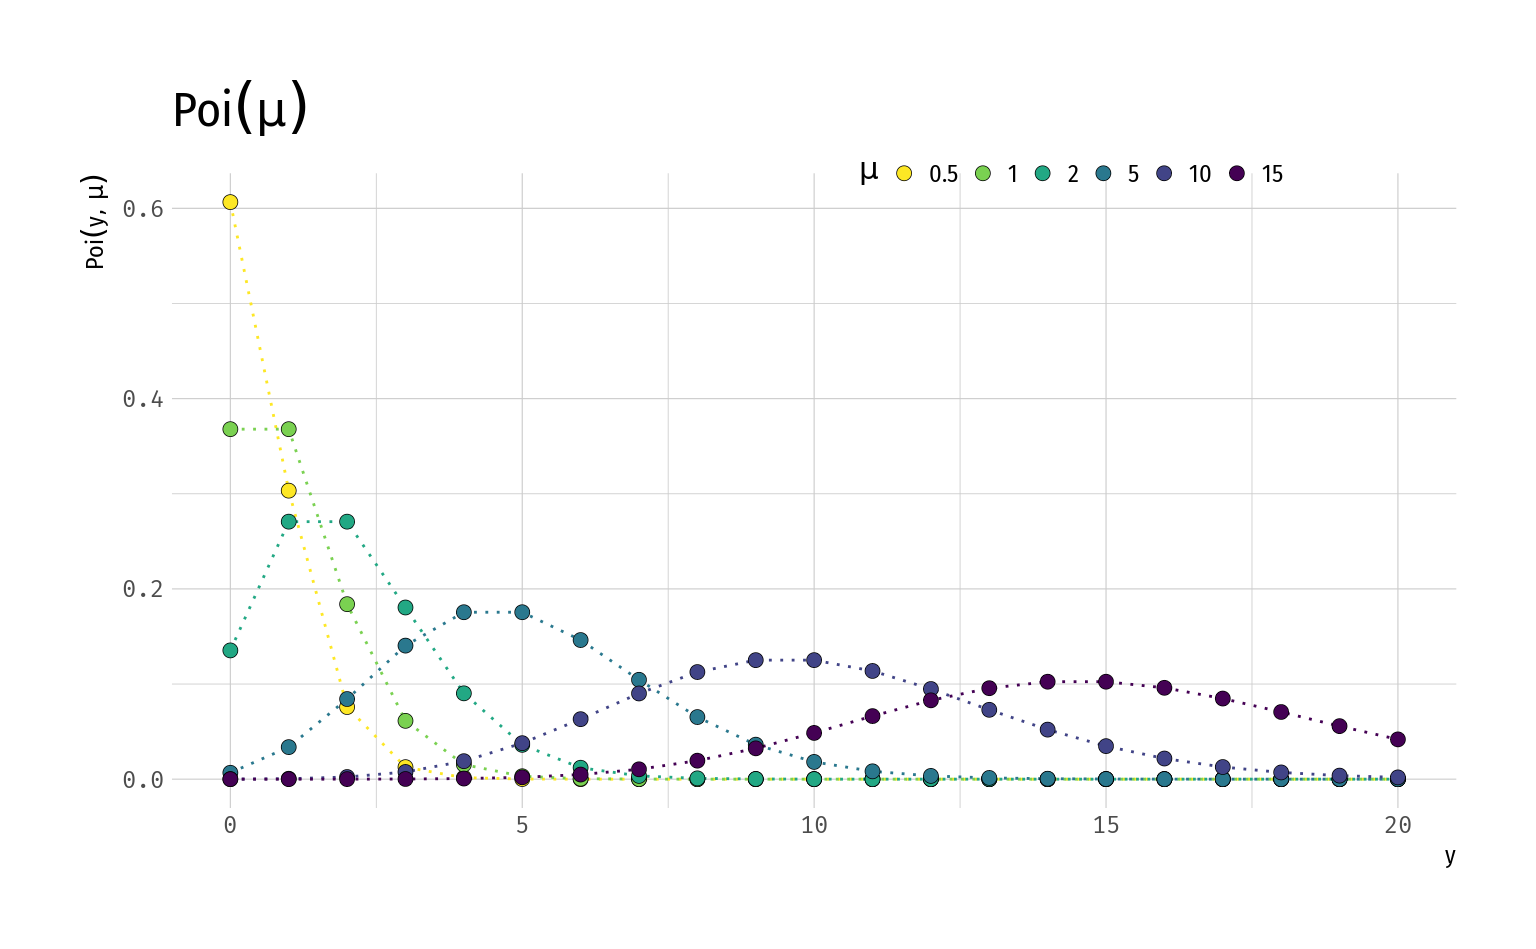
\includegraphics{poisson-regression_files/figure-latex/poissondists-1} 

}

\caption{Poisson-Verteilungen mit ausgewählten Parametern.}\label{fig:poissondists}
\end{figure}

\BeginKnitrBlock{definition}[Poisson-Modell]
\protect\hypertarget{def:poisson-modell}{}{\label{def:poisson-modell} \iffalse (Poisson-Modell) \fi{} }Die Zielvariablen \(y_i \in \mathbb{N}_0\) sind (bedingt) unabhängig gegeben der Kovariablen \(x_{i1}, x_{i2}, \ldots, x_{ik}\).

Die Rate \(\mu_i = \mathbb{E}(y_i\ |\ \mathbf{x}_i)\) der Poissonverteilung wird in der Regel log-linear modelliert als

\begin{align*}
  \log(\mu_i) &= \eta_i 
    = \mathbf{x}_i^\prime \boldsymbol{\beta} 
    = \beta_0 + \beta_1 x_1 + \ldots + \beta_k x_{ik} \\
  \mu_i &= \exp(\eta_i) 
    = \exp(\beta_0) \cdot \exp(\beta_1 x_1) \cdot \ldots \cdot \exp(\beta_k x_k)
\end{align*}
\EndKnitrBlock{definition}

Vgl. \citet{fahrmeirRegressionModelleMethoden2009}

Für das log-lineare Poisson-Modell entsprechen die resultierenden Koeffizienten der Veränderung der log-counts -- durch Exponentiation lassen diese sich als \emph{incidence rate ratios} (\emph{IRR}) interpretieren.

Um auf ungleiche Expositionsdauern oder -gebiete zu adjustieren wird ein \textbf{offset} (oder auch \emph{exposure}) benötigt. Dazu dient der Koeffizient \(t\), der die Länge der Zeit unter Exposition angibt:

\begin{equation}
f(y, \mu) = \frac{\exp(\mu) (t \mu)^y}{y!}
\end{equation}

Damit entspricht \(t \mu\) der Inzidenzrate des Outcomes adjustiert auf e.g.~die geographische Lage oder Expositionsdauer. Ohne Offset entspräche \(t = 1\).
Für als Offset wird in der Regel \(\log(t)\) verwendet, womit gelten:

\begin{align*}
\hat{\mu} &= \exp{x \boldsymbol{\beta} + \log(t)} \\
\Leftrightarrow \exp(x \boldsymbol{\beta}) &= \frac{\hat{\mu}}{t} \\
\Leftrightarrow \hat{\mu} &= t \exp(x \boldsymbol{\beta})
\end{align*}

Ein offset kann z.B. in \texttt{R} via \texttt{+\ offset(log(variable))} in der model \texttt{formula} oder über das Argument \texttt{offset\ =\ log(variable)} in \texttt{glm} und verwandten Funktionen angegeben werden.

\hypertarget{annahmen}{%
\subsection{Annahmen}\label{annahmen}}

\begin{enumerate}
\def\labelenumi{\arabic{enumi}.}
\tightlist
\item
  Die Abhängige / Zielvariable \(Y\) muss eine Zählung sein, i.e.~die Verteilung ist diskret mit einem einzelnen Parameter \(\mu\) der Poisson-Verteilung für Erwartungswert und Varianz.
\item
  \(y \in \mathbb{N}_0\), insbesondere: \(Y\) muss 0 enthalten \emph{können} (siehe auch \ref{trunc-cens} \protect\hyperlink{trunc-cens}{Truncation und Censoring})
\item
  Beobachtungen sind \emph{unabhängig}, i.e.~weder longitudinal noch gepoolt.

  \begin{itemize}
  \tightlist
  \item
    Möglicher Test durch Vergleich der Modell-SE und der SE adjustiert durch robuste sandwich-estimators (siehe \ref{sandwich}): Große Unterschiede implizieren korrelierte Daten
  \end{itemize}
\item
  Balanced: Die Zellen sind in etwa so besetzt wie es aufgrund der Poissonverteilung erwartet wird.
\item
  Erwartungswert und Varianz sind identisch (\emph{equidispersion}), i.e.~ein größerer Erwartungswert impliziert auch eine größere Varianz (siehe \ref{dispersion}).
\item
  Die \(\chi^2\)-Statistik hat einen Wert nahe 1, i.e.~beobachtete und erwartete Varianzen der response sind gleich (Dispersionsindex).
\end{enumerate}

(Nach Tabelle in \citep{hilbeModelingCountData2014}, braucht noch Deduplizierung)

Alternative Formulierung nach \citet{winkelmannEconometricAnalysisCount2010} (p.~64):

\begin{enumerate}
\def\labelenumi{\arabic{enumi}.}
\tightlist
\item
  \(f(y\ |\ \mu) = \frac{e^{-\mu} \mu^y}{y!} \quad \mu > 0, y = 0, 1, 2, \ldots\).
\item
  \(\mu = \exp(\mathbf{x}' \boldsymbol{\beta})\).
\item
  Beobachtungspaare \((y_i, x_i)\) sind unabhängig verteilt.
\end{enumerate}

\hypertarget{dispersion}{%
\subsection{Dispersion}\label{dispersion}}

\BeginKnitrBlock{definition}[Equi-, Extra-, Over-, Underdispersion]
\protect\hypertarget{def:def-dispersions}{}{\label{def:def-dispersions} \iffalse (Equi-, Extra-, Over-, Underdispersion) \fi{} }Für Zählvariablen \(y_i \in \mathbb{N}_0\) und erklärenden Variablen \(\mathbf{x}_i\) gilt innerhalb eines Modells:

\begin{align*}
\text{Equdispersion:}  \quad & \mathrm{Var}(y_i) = \mathrm{Var}(y_i\ |\ \mathbf{x}_i) \\
\text{Extradispersion:}\quad & \mathrm{Var}(y_i) \neq \mathrm{Var}(y_i\ |\ \mathbf{x}_i) \\
\text{Overdispersion:} \quad & \mathrm{Var}(y_i) > \mathrm{Var}(y_i\ |\ \mathbf{x}_i) \\
\text{Underdispersion:}\quad & \mathrm{Var}(y_i) < \mathrm{Var}(y_i\ |\ \mathbf{x}_i)
\end{align*}
\EndKnitrBlock{definition}

\BeginKnitrBlock{definition}[Poisson-Overdispersion]
\protect\hypertarget{def:def-pois-overdispersion}{}{\label{def:def-pois-overdispersion} \iffalse (Poisson-Overdispersion) \fi{} }Innerhalb eines Poisson-Modells (vgl. Abschnitt \ref{poisson-modell}) mit der Annahme

\begin{align*}
y_i\ |\ \mathbf{x}_i &\sim \mathrm{Poi}(\mu_i) \\[1.5em]
\mu &= \mathbb{E}(y_i\ |\ \mathbf{x}_i) = \mathrm{Var}(y_i\ |\ \mathbf{x}_i) \quad \text{(Equidispersion)}
\end{align*}

spricht man von \textbf{Poisson-Overdispersion} wenn die Varianz der Beobachtungen die erwartete Varianz des Poisson-Modells übersteigt:

\begin{equation*}
  \mathrm{Var}(y_i\ |\ \mathbf{x}_i) > \mathbb{E}(y_i\ |\ \mathbf{x}_i)
\end{equation*}

in einem Modell mit overdispersion gilt die Annahme:

\begin{equation*}
  \mathrm{Var}(y_i\ |\ \mathbf{x}_i) = \theta \cdot \mu_i
\end{equation*}

Mit \emph{Dispersionsparameter} \(\theta\) \citep[vgl.][p.~210]{fahrmeirRegressionModelleMethoden2009}
\EndKnitrBlock{definition}

Als Dispersionsstatistik können \emph{deviance dispersion} oder \emph{Pearson dispersion} berechnet werden. Laut \citet{hilbeModelingCountData2014} ist die \emph{Pearson dispersion} zu bevorzugen, da sie für echte Poisson-Modelle gleich 1 ist, wohingegen die \emph{deviance dispersion} nach oben verzerrt ist.

\BeginKnitrBlock{definition}[Pearson-Dispersion]
\protect\hypertarget{def:def-pearsondisp}{}{\label{def:def-pearsondisp} \iffalse (Pearson-Dispersion) \fi{} }Nach \citet{hilbeModelingCountData2014} (p.~77ff):

Die Pearson \(\chi^2\)-Statistik ist die Summe der quadrierten (Pearson-)Residuen gewichtet mit der Modellvarianz:

\begin{equation*}
\chi_{\text{Pearson}}^2 = \sum_{i=1}^n \frac{(y_i - \hat{\mu}_i)^2}{\mathrm{Var}(\hat{\mu}_i)}
\end{equation*}

und die \textbf{Pearson-Dispersionsstatistik}:

\begin{equation*}
D = \frac{\chi_{\text{Pearson}}^2}{\mathrm{df}}
\end{equation*}

Mit der Interpretation

\begin{equation*}
\mathrm{D} =
  \begin{cases}
    < 1 & \Longrightarrow \text{Underdispersion} \\
      1 & \Longrightarrow \text{Equidispersion (Poisson)} \\
    > 1 & \Longrightarrow \text{Overdispersion}
  \end{cases}
\end{equation*}

Für Modelle moderater Größe kann man ab Werten über 1.25 von overdispersion sprechen, wobei für große Stichproben auch schon ab 1.05 overdispersion vorliegen kann -- zumindest nach \citet{hilbeModelingCountData2014} (p.~82), der aber leider keine konkreten Angaben für seine Definition von \enquote{moderaten} oder \enquote{großen} Stichproben macht.
\EndKnitrBlock{definition}

In \texttt{R} kann die Pearson-Dispersion wie folgt berechnet werden:

\begin{Shaded}
\begin{Highlighting}[]
\CommentTok{# Model fit}
\NormalTok{mod <-}\StringTok{ }\KeywordTok{glm}\NormalTok{(y }\OperatorTok{~}\StringTok{ }\NormalTok{x1 }\OperatorTok{+}\StringTok{ }\NormalTok{x2 }\OperatorTok{+}\StringTok{ }\NormalTok{x3, }\DataTypeTok{data =}\NormalTok{ sim, }\DataTypeTok{family =} \KeywordTok{poisson}\NormalTok{(}\DataTypeTok{link =} \StringTok{"log"}\NormalTok{))}

\CommentTok{# Pearson dispersion}
\KeywordTok{sum}\NormalTok{(}\KeywordTok{resid}\NormalTok{(mod, }\DataTypeTok{type =} \StringTok{"pearson"}\NormalTok{)}\OperatorTok{^}\DecValTok{2}\NormalTok{) }\OperatorTok{/}\StringTok{ }\NormalTok{mod}\OperatorTok{$}\NormalTok{df.residual}
\end{Highlighting}
\end{Shaded}

\ldots{}wofür wir in Abschnitt \ref{helperfuns} eine Hilfsfunktion \texttt{dispersion()} definiert haben.

\hypertarget{overdispersion}{%
\subsubsection{Overdispersion}\label{overdispersion}}

Der vermutlich häufigste Fall für Count-Daten: Die Varianz der abhängigen Variable ist größer als ihr Erwartungswert, bzw. größer als ihre erwartete Varianz innerhalb eines Modells.
\citet{hilbeModelingCountData2014} unterscheidet zwischen echter und scheinbarer (\emph{apparent}) Overdispersion, wobei letztere oft durch geeignete Korrekturen kompensiert werden kann, wobei \emph{echte} Overdisperion sowohl Parameterschätzung als auch Modellanpassung im Allgemeinen beeinträchtigt.

Nach \citet{hilbeModelingCountData2014} (p.~82) entsteht \emph{echte} Overdispersion durch:

\begin{itemize}
\tightlist
\item
  Positive Korrelation zwischen responses
\item
  Große Variation zwischen response-probabilities und counts
\item
  Verletzungen der Verteilungsannahme (i.e.~Poissonverteilung)
\item
  \enquote{Proneness}: Frühere Ereignisse beeinflussen das Auftreten späterer Ereignisse \footnote{Diese Annahme (Unabhängigkeit der Ereignisse) der Poissonverteilung ist auch der Grund, warum sich die Poissonverteilung prinzipiell \textbf{nicht} eignet um Epidemien wie Ebola zu modellieren. Freundliche Grüße an Frau Pigeot, \enquote{Statistische Modellierung I}, WiSe 18/19.}
\end{itemize}

Ursachen für \emph{scheinbare} (\emph{apparent}), und damit (bedingt) korrigierbare Overdispersion nach \citet{hilbeModelingCountData2014} (p.~41, 82):

\begin{enumerate}
\def\labelenumi{\arabic{enumi}.}
\tightlist
\item
  Fehlende explanatorische Prädiktoren
\item
  Ausreißer
\item
  Fehlende Interaktionsterme
\item
  Ein Prädiktor muss transformiert werden
\item
  Die Daten sind zu dünn besetzt (\emph{sparse})
\item
  Fehlende Werte, die nicht zufällig sind (missing not at random, \emph{MNAR} -- siehe auch Anhang \ref{appendix-missingness}
\end{enumerate}

Ein einfaches simuliertes Beispiel zur Auswirkung von fehlenden Prädiktoren:

\begin{Shaded}
\begin{Highlighting}[]
\CommentTok{# Generate binary variable in [0, 1] with a given proportion of 1's}
\NormalTok{rbinary <-}\StringTok{ }\ControlFlowTok{function}\NormalTok{(n, }\DataTypeTok{prob =} \FloatTok{0.5}\NormalTok{) \{}
  \KeywordTok{sample}\NormalTok{(}\DecValTok{0}\OperatorTok{:}\DecValTok{1}\NormalTok{, }\DataTypeTok{size =}\NormalTok{ n, }\DataTypeTok{replace =} \OtherTok{TRUE}\NormalTok{, }\DataTypeTok{prob =} \KeywordTok{c}\NormalTok{(}\DecValTok{1} \OperatorTok{-}\StringTok{ }\NormalTok{prob, prob))}
\NormalTok{\}}

\KeywordTok{set.seed}\NormalTok{(}\DecValTok{436}\NormalTok{)}
\NormalTok{n <-}\StringTok{ }\DecValTok{1000}

\NormalTok{sim <-}\StringTok{ }\KeywordTok{tibble}\NormalTok{(}
  \DataTypeTok{x1 =} \KeywordTok{rbinary}\NormalTok{(n, }\FloatTok{.1}\NormalTok{),}
  \DataTypeTok{x2 =} \KeywordTok{rbinary}\NormalTok{(n, }\FloatTok{.2}\NormalTok{),}
  \DataTypeTok{x3 =} \KeywordTok{rbinary}\NormalTok{(n, }\FloatTok{.3}\NormalTok{),}
  \DataTypeTok{eta =} \FloatTok{0.5} \OperatorTok{+}\StringTok{ }\DecValTok{1} \OperatorTok{*}\StringTok{ }\NormalTok{x1 }\OperatorTok{+}\StringTok{ }\DecValTok{2} \OperatorTok{*}\StringTok{ }\NormalTok{x2 }\OperatorTok{+}\StringTok{ }\FloatTok{0.5} \OperatorTok{*}\StringTok{ }\NormalTok{x3,}
  \DataTypeTok{mu =} \KeywordTok{exp}\NormalTok{(eta),}
  \DataTypeTok{py =} \KeywordTok{rpois}\NormalTok{(n, mu)}
\NormalTok{)}

\CommentTok{# Korrektes modell:}
\NormalTok{mod <-}\StringTok{ }\KeywordTok{glm}\NormalTok{(py }\OperatorTok{~}\StringTok{ }\NormalTok{x1 }\OperatorTok{+}\StringTok{ }\NormalTok{x2 }\OperatorTok{+}\StringTok{ }\NormalTok{x3, }\DataTypeTok{data =}\NormalTok{ sim, }\DataTypeTok{family =} \KeywordTok{poisson}\NormalTok{(}\DataTypeTok{link =} \StringTok{"log"}\NormalTok{))}
\KeywordTok{dispersion}\NormalTok{(mod)}
\end{Highlighting}
\end{Shaded}

\begin{verbatim}
#> X-squared(996) = 1029.70
#> Pearson Dispersion = 1.034
\end{verbatim}

\begin{Shaded}
\begin{Highlighting}[]
\CommentTok{# Modell mit fehlendem Prädiktor:}
\NormalTok{mod2 <-}\StringTok{ }\KeywordTok{glm}\NormalTok{(py }\OperatorTok{~}\StringTok{ }\NormalTok{x1 }\OperatorTok{+}\StringTok{ }\NormalTok{x3, }\DataTypeTok{data =}\NormalTok{ sim, }\DataTypeTok{family =} \KeywordTok{poisson}\NormalTok{(}\DataTypeTok{link =} \StringTok{"log"}\NormalTok{))}
\KeywordTok{dispersion}\NormalTok{(mod2)}
\end{Highlighting}
\end{Shaded}

\begin{verbatim}
#> X-squared(997) = 7669.65
#> Pearson Dispersion = 7.693
\end{verbatim}

\hypertarget{underdispersion}{%
\subsubsection{Underdispersion}\label{underdispersion}}

Underdispersion ist der Fall, wenn vorliegende Daten eine geringere Varianz aufweisen, als auf Basis eines Poisson-Modells erwartet würde, das heißt die Daten sind \enquote{enger zusammengeklumpt}.
Bei underdispersion werden die Standardfehler des Modells \emph{über}schätzt, im Gegensatz zur overdispersion, bei der Standardfehler \emph{unter}schätzt werden \citep[p.~210]{hilbeModelingCountData2014}.

Im Allgemeinen wird für diese Situation die \href{https://stats.stackexchange.com/a/237177/80056}{generalized Poisson empfohlen} \citep{hilbeModelingCountData2014}, da diese Erweiterung der Poisson-Verteilung nicht nur einen zusätzlichen Parameter für die Varianz hat (analog NB, PIG), sondern dieser Parameter auch negativ sein kann.

Weiterhin taucht im Kontext von hurdle models (siehe \ref{mod-hurdle}) folgende Bemerkung auf:

\begin{quote}
{[}\ldots{}{]} that underdispersion occurs if \textbf{zeros are less frequent than the parent distribution would predict}.
The higher the expected value of the Poisson distribution, the lower the predicted probability of zero outcome and the lower the scope for underdispersion.
-- \citep[p.~180 (eigene Hervorhebung)]{winkelmannEconometricAnalysisCount2010}
\end{quote}

Daraus lässt sich auch schließen, dass in Situationen mit binären outcomes und sehr niedrigem Erwartungswert die erwartete Anzahl an Nullen sehr hoch sein wird -- weshalb es an dieser Stelle vermutlich eine Überlappung zwischen underdispersion und zero-inflation gibt.

\hypertarget{multiparam}{%
\section{Mehrparametrische Modelle}\label{multiparam}}

\begin{figure}

{\centering \includegraphics{poisson-regression_files/figure-latex/model-graph-1} 

}

\caption{Hierarchie ausgewählter Count-Modelle. In Klammern: Zu schätzende Parameter der zugrundeliegenden Verteilung}\label{fig:model-graph}
\end{figure}

Zweiparametrische Modelle haben neben dem Parameter für den Erwartungswert einen weiteren Parameter für die Dispersion, was wir natürlich insbesondere im Kontext der Dispersionsproblematik sehr nützlich finden.\\
Alle hier aufgeführten Modelle (inklusive der zero-inflation models) können als Verallgemeinerung der Poisson-Verteilung um (mindestens) einen weiteren Parameter aufgefasst werden. Die Unterschiede liegen hauptsächlich in der Parametrisierung und den damit zusammenhängenden Einschränkungen. Die \emph{Negative Binomialverteilung} und die \emph{Poisson Inverse Gaussian} zum Beispiel erweitern beide die Poisson um einen Dispersionsparameter, machen aber unterschiedliche Annahmen zur Verteilung der Varianz (gamma- vs.~invers-normalverteilt).

Tabelle \ref{tab:modelstable} zeigt eine Reihe von Verteilungen mit entsprechend parametrisierter Varianz abhängig vom Erwartungswert \(\mu\) und einem Dispersionsparameter \(\alpha\).

\begin{table}[t]

\caption{\label{tab:modelstable} Ein Überblick einiger Modelle mit Varianzparametrisierung (nach @hilbeModelingCountData2014, p. 12).}
\centering
\begin{tabular}{lll}
\toprule
Model & Mean & Variance\\
\midrule
Poisson & $\mu$ & $\mu$\\
Negative Binomial I (NB1) & $\mu$ & $\mu (1 + \alpha) = \mu + \alpha\mu$\\
Negative Binomial II (NB2) & $\mu$ & $\mu (1 + \alpha\mu) = \mu + \alpha\mu^2$\\
Negative Binomial-P (NBP) & $\mu$ & $\mu (1 + \alpha\mu^p) = \mu + \alpha\mu^p$\\
Poisson Inverse Gaussian (PIG) & $\mu$ & $\mu (1 + \alpha\mu^2) = \mu + \alpha\mu^3$\\
Generalized Poisson (GP) & $\mu$ & $\mu (1 + \alpha\mu)^2 = \mu + 2\alpha\mu^3 + \alpha^2\mu^3$\\
\bottomrule
\end{tabular}
\end{table}

\hypertarget{mod-nb}{%
\subsection{Negativ Binomial (NB)}\label{mod-nb}}

Die Negative Binomialverteilung (\emph{NB}) kann als zweiparametrische Erweiterung der \emph{Poisson} betrachtet werden, wobei die Varianz (separat vom Erwartungswert) als Gamma-verteilte Zufallsvariable betrachtet wird (\emph{Poisson-Gamma Mischmodell}).\\
Für eine ausführliche Beschreibung, siehe \citet{hilbeModelingCountData2014} (p.~126ff).

\BeginKnitrBlock{definition}[Negative Binomialverteilung]
\protect\hypertarget{def:defNB}{}{\label{def:defNB} \iffalse (Negative Binomialverteilung) \fi{} }Nach \citet{perumean-chaneyZeroinflatedOverdispersedWhat2013} (p.~1675):

Für \(Y \sim NB(\mu, \theta)\) gilt

\begin{equation}
P(Y = y) = \frac{\Gamma(\theta + y)}{\Gamma(\theta) \Gamma(y+1)} \frac{\theta^\theta \mu^y}{(\theta + \mu)^{(\theta + y)}}, \quad y = 0, 1, 2, \ldots
\end{equation}

Mit \(\mathbb{E}(Y) = \mu\) und \(\mathrm{Var}(Y) = \mu + \frac{\mu^2}{\theta}\)
\EndKnitrBlock{definition}

Für eine alternative Darstellung unter Verwendung von \(\alpha = \frac{1}{\theta}\), siehe \citet{hilbeModelingCountData2014} (p.~130)

Der gängigste Anwendungsfall der \emph{NB} findet sich bei Daten mit nicht korrigierbarer overdispersion (siehe Abschnitt \ref{overdispersion}), da der Parameter \(\theta\) bzw. auch \(\alpha = \frac 1 \theta\) als \emph{Dispersionsparameter} dient:

\BeginKnitrBlock{definition}[NB-Dispersionsparameter]
\protect\hypertarget{def:nbdisppar}{}{\label{def:nbdisppar} \iffalse (NB-Dispersionsparameter) \fi{} }
Meist wird der Parameter als \(\alpha\) bezeichnet, mit der Interpretation (relativ zum Poisson-Modell):

\[\mathrm{Var}(Y) = \mu + \alpha \mu^2\]

\begin{align}
  \alpha &= 0 &&\Longrightarrow \text{ Äquivalent zur Poissonverteilung} \\
  \alpha &> 0 &&\Longrightarrow \text{ Overdispersion}
\end{align}

Je nach Quelle (und unter Anderem in R (z.B. \texttt{MASS::glm.nb})) wird die inverse Variante \(\theta = \frac 1 \alpha\) verwendet, womit gilt:

\[\mathrm{Var}(Y) = \mu + \frac{\mu^2}{\theta}\]

\begin{align}
  \theta &> 0 &&\Longrightarrow \text{ Overdispersion} \\
  \theta &\to \infty &&\Longrightarrow \text{ Äquivalent zur Poissonverteilung}
\end{align}

Siehe dazu auch \citet{hilbeModelingCountData2014} (p.~131).
\EndKnitrBlock{definition}

Das GLM sieht keinen weiteren zu schätzenden Parameter vor, weshalb \(\theta\) bzw. \(\alpha\) in der Praxis separat geschätzt wird.\\
Der wohl wichtigste Aspekt des Dispersionsparameters, unabhängig davon ob \(\alpha\) oder \(\theta\) verwendet wird, ist sein Vorzeichen: Er ist \emph{immer} positiv, das heißt die Varianz der NB ist entweder \emph{größer oder gleich} der Poisson, oder mit anderen Worten:

\begin{quote}
\enquote{The negative binomial model adjusts for Poisson overdispersion; it \textbf{cannot be used to model underdispersed} Poisson data}

--- \citep[ (p.~11), eigene Hervorhebung]{hilbeModelingCountData2014}
\end{quote}

Je nach Software/Algorithmus ist es auch möglich, dass ein NB-fit nicht möglich ist, wenn \(\alpha \approx 0\) (die Verteilung zu nah an Poisson) bzw. die Daten Poisson-underdispersed sind.

Weiterhin gibt es zwei verschiedene Formulierungen der Negativen Binomialverteilung, NB1 und NB2, deren Nummerierung auf den Exponenten im zweiten Term ihrer Varianzen zurückzuführen ist:

\BeginKnitrBlock{definition}[NB1 und NB2]
\protect\hypertarget{def:defNB1NB2}{}{\label{def:defNB1NB2} \iffalse (NB1 und NB2) \fi{} }Nach \citet{hilbeModelingCountData2014} (p.~126f):

Die \textbf{NB1}, oder auch \emph{lineare} Negative Binomialverteilung hat die Varianz

\begin{equation*}
\mathrm{Var}(Y) = \mu + \alpha \mu
\end{equation*}

\ldots{}und die gängigere \textbf{NB2}, oder auch \emph{quadratische} Negative Binomialverteilung hat (wie oben beschrieben) die Varianz

\begin{equation*}
\mathrm{Var}(Y) = \mu + \alpha \mu^2
\end{equation*}
\EndKnitrBlock{definition}

Beide Varianten können wie MLE geschätzt werden, wobei NB2 zusätzlich im Kontext des GLM via IRLS geschätzt werden kann.

Als link wird \(\log \mu\) verwendet, wobei der \emph{canonical link} eigentlich \(\log\left(\frac{\alpha\mu}{1 + \alpha\mu}\right)\) ist \footnote{Daher können Standardfehler nicht wie für canonical models überlich via OIM (\emph{observed information matrix}), sondern via EIM (\emph{expected information matrix}) geschätzt werden. Die EIM-Methode liefert weniger genaue Resultate für kleine Stichproben (n \textless{} 30).}.

Für ein gut angepasstes NB-Modell gilt analog eines Poisson-Modells, dass die Dispersionsstatistik approximativ 1 ist (siehe \ref{def:def-pearsondisp}).

Zur Anwendung in R gibt es zwei Möglichkeiten: \texttt{MASS::glm.nb} oder \texttt{msme::nbinomial}, wobei letztere mehrere Optionen zur Parametrisierung hat und zusätzlich die Dispersionsstatistik ausgibt:

\begin{Shaded}
\begin{Highlighting}[]
\NormalTok{mod_nb <-}\StringTok{ }\NormalTok{MASS}\OperatorTok{::}\KeywordTok{glm.nb}\NormalTok{(docvis }\OperatorTok{~}\StringTok{ }\NormalTok{outwork }\OperatorTok{+}\StringTok{ }\NormalTok{age,}
                       \DataTypeTok{data =}\NormalTok{ rwm1984)}
\KeywordTok{summary}\NormalTok{(mod_nb)}
\end{Highlighting}
\end{Shaded}

\begin{verbatim}
#> 
#> Call:
#> MASS::glm.nb(formula = docvis ~ outwork + age, data = rwm1984, 
#>     init.theta = 0.4353451729, link = log)
#> 
#> Deviance Residuals: 
#>     Min       1Q   Median       3Q      Max  
#> -1.5316  -1.2816  -0.4895   0.1043   5.0468  
#> 
#> Coefficients:
#>              Estimate Std. Error z value Pr(>|z|)    
#> (Intercept) -0.039550   0.106669  -0.371    0.711    
#> outwork      0.414662   0.055451   7.478 7.55e-14 ***
#> age          0.022146   0.002396   9.242  < 2e-16 ***
#> ---
#> Signif. codes:  0 '***' 0.001 '**' 0.01 '*' 0.05 '.' 0.1 ' ' 1
#> 
#> (Dispersion parameter for Negative Binomial(0.4353) family taken to be 1)
#> 
#>     Null deviance: 4100.8  on 3873  degrees of freedom
#> Residual deviance: 3909.6  on 3871  degrees of freedom
#> AIC: 16674
#> 
#> Number of Fisher Scoring iterations: 1
#> 
#> 
#>               Theta:  0.4353 
#>           Std. Err.:  0.0135 
#> 
#>  2 x log-likelihood:  -16665.5250
\end{verbatim}

\begin{Shaded}
\begin{Highlighting}[]
\NormalTok{mod_nb2 <-}\StringTok{ }\NormalTok{msme}\OperatorTok{::}\KeywordTok{nbinomial}\NormalTok{(docvis }\OperatorTok{~}\StringTok{ }\NormalTok{outwork }\OperatorTok{+}\StringTok{ }\NormalTok{age,}
                           \DataTypeTok{data =}\NormalTok{ rwm1984)}
\KeywordTok{summary}\NormalTok{(mod_nb2)}
\end{Highlighting}
\end{Shaded}

\begin{verbatim}
#> 
#> Call:
#> ml_glm2(formula1 = formula1, formula2 = formula2, data = data, 
#>     family = family, mean.link = mean.link, scale.link = scale.link, 
#>     offset = offset, start = start, verbose = verbose)
#> 
#> Deviance Residuals:
#>    Min. 1st Qu.  Median    Mean 3rd Qu.    Max. 
#> -1.5320 -1.2816 -0.4896 -0.4553  0.1035  5.0497 
#> 
#> Pearson Residuals:
#>      Min.   1st Qu.    Median      Mean   3rd Qu.      Max. 
#> -0.637147 -0.607737 -0.376257  0.000055  0.108975 21.659334 
#> 
#> Coefficients (all in linear predictor):
#>               Estimate      SE      Z         p     LCL    UCL
#> (Intercept)    -0.0443 0.10570 -0.419     0.675 -0.2514 0.1629
#> outwork         0.4141 0.05532  7.485  7.15e-14  0.3056 0.5225
#> age             0.0223 0.00237  9.401  5.42e-21  0.0176 0.0269
#> (Intercept)_s   2.2971 0.07098 32.364 8.85e-230  2.1580 2.4362
#> 
#> Null deviance: 4100.786  on  3872 d.f.
#> Residual deviance: 3909.522  on  3870 d.f.
#> Null Pearson: 5835.302  on  3872 d.f.
#> Residual Pearson: 5458.2  on  3870 d.f.
#> Dispersion: 1.410388
#> AIC:  16673.53
#> 
#> Number of optimizer iterations:  82
\end{verbatim}

\hypertarget{mod-pig}{%
\subsection{Poisson Inverse Gaussian (PIG)}\label{mod-pig}}

So wie die \emph{NB} als mixture aus Poisson-Verteilung mit Gamma-verteilter Varianz betrachtet werden kann, ist die \emph{Poisson Inverse Gaussian} (\emph{PIG}) eine mixture aus Poisson-Verteilung mit \href{https://en.wikipedia.org/wiki/Inverse_Gaussian_distribution}{invers-normalverteilter} Varianz. Demnach kann man \emph{PIG} als Alternative zur \emph{NB} verwenden, insbesondere für den Fall sehr rechtsschiefer Daten.

\begin{quote}
\enquote{Simply put, PIG models can better deal with highly overdispersed data that can negative binomial regression, particularly data clumped heavily at 1 and 2}

-- \citet{hilbeModelingCountData2014} (p.~163)
\end{quote}

\textbf{Software}:

\begin{itemize}
\tightlist
\item
  R: \texttt{gamlss} (CRAN)
\item
  SAS: Machbar via \texttt{NLMIXED}, aber unschön \citep[siehe][]{high2018AlternativeVariance}.
\item
  Stata: \texttt{pigreg}
\end{itemize}

\hypertarget{mod-gp}{%
\subsection{Generalized Poisson (GP)}\label{mod-gp}}

Die Verteilung besitzt auch einen zusätzlichen Dispersionsparameter (analog NB, PIG), allerdings kann dieser hier auch negative Werte annehmen, womit die GP für alle Dispersionsarten (bzw. insbesondere underdispersion) geeignet ist.

\BeginKnitrBlock{definition}[Generalized Poisson]
\protect\hypertarget{def:def-genois}{}{\label{def:def-genois} \iffalse (Generalized Poisson) \fi{} }Aus \citet{hilbeModelingCountData2014} (p.~211) und \citet{harris2012ModelingUnderdispersed}:

Eine Variable \(Y\) ist \emph{generalized Poisson} verteilt mit der PMF:

\begin{equation*}
P(Y = y_i) = \frac{\theta_i \left(\theta_i + \delta y_i\right)^{y_i - 1}}{y_i !} \exp(-\theta_i - \delta y_i), \quad y_i = 1, 2, 3, \ldots
\end{equation*}

\begin{align*}
\theta_i > 0, \quad \max(-1, \frac{-\theta_i}{4}) < \delta < 1 \\[2em]
\mu_i = \mathbb{E}(Y_i) &= \frac{\theta_i}{1 - \delta} \\
\mathrm{Var}(Y_i) &= \frac{\theta}{(1 - \delta)^3} 
                   = \frac{1}{(1 - \delta)^2} \mathbb{E}(Y_i)
                   = \Phi \mathbb{E}(Y_i)
\end{align*}

Wobei \(\Phi = \frac{1}{(1 - \theta)^2}\) als Dispersionsparameter dient.

Es gilt außerdem

\begin{align*}
\delta = 0 &\Longrightarrow \text{Equidispersion (Poisson)} \\
\delta < 0 &\Longrightarrow \text{Underdispersion} \\
\delta > 0 &\Longrightarrow \text{Overdispersion}
\end{align*}

Auch hier kann ein Likelihood-Ratio Test auf \(\delta = 0\) durchgeführt werden, analog \(\alpha = 0\) für die NB -- wobei \(\delta\) hier keine Restriktion hat (siehe BLR, Definition \ref{def:BLR}).
\EndKnitrBlock{definition}

\textbf{Software}:

\begin{itemize}
\tightlist
\item
  R: \texttt{VGAM}: \texttt{vgam(...,\ family\ =\ genpoisson())}{]}

  \begin{itemize}
  \tightlist
  \item
    Hier wird das obige \(\delta\) als \(\lambda\) bezeichnet (Verwechslungsgefahr mit Poisson-Parameter)
  \item
    Numerisch instabil für \(\lambda\) nahe 0 oder 1
  \item
    Siehe \href{https://rdrr.io/cran/VGAM/man/genpoisson.html}{\texttt{?VGAM::genpoisson}}
  \end{itemize}
\item
  Alternativ via \href{https://www.gamlss.com/}{gamlss}: \texttt{gamlss(...,\ family\ =\ GPO)}
\end{itemize}

In beiden R-Varianten habe ich bisher nicht geschafft \(\theta\), den Dispersionsparameter, zu extrahieren -- auch wenn die Koeffizientien aus dem Stata-Beispiel in \citep[p.~213f]{hilbeModelingCountData2014} reproduzierbar sind.

\begin{itemize}
\tightlist
\item
  SAS: \texttt{NLMIXED} oder \texttt{FMM}, siehe auch \href{http://support.sas.com/kb/56/549.html}{SAS support document}
\end{itemize}

Allgemein scheint die Parametrisierung (und Notation der Parameter) zu variieren.

\hypertarget{mod-comp}{%
\subsection{Conway-Maxwell Poisson (COMP)}\label{mod-comp}}

\BeginKnitrBlock{definition}[Conway-Maxwell-Poisson Modell (CMP)]
\protect\hypertarget{def:unnamed-chunk-2}{}{\label{def:unnamed-chunk-2} \iffalse (Conway-Maxwell-Poisson Modell (CMP)) \fi{} }Nach \citet{shmueli2005UsefulDistribution} (p.~129):

\begin{align}
P(X = x) &= \frac{\lambda^x}{(x!)^\nu} \frac{1}{Z(\lambda, \nu)}, \quad x = 0, 1, 2, \ldots \\
Z(\lambda, \nu) &= \sum_{j = 0}^\infty \frac{\lambda^j}{(j!)^\nu} \\
\\
\lambda > 0&, \nu \ge 0
\end{align}

Mit (im Unterschied zur Poisson) nichtlinearer Zerfallsrate \(\nu\) \emph{rate of decay}, so dass:

\begin{equation}  
\frac{P(X = x -1)}{P(X = x)} = \frac{x^\nu}{\lambda}
\end{equation}

Der Zusammenhang zwischen \(\nu\) und \(\lambda\) nach \citet{sellers2010FlexibleRegression} (p.~946) legt Nahe, dass \(\nu\) ähnlich \(\alpha\) in NB-Modellen die Dispersion bestimmt:

\begin{align*}
  \mathrm{Var}(Y_i) =& \lambda_i \frac{\partial}{\partial \lambda_i} \mathbb{E}(Y_i)
            \approx \lambda_i \frac{\partial}{\partial \lambda_i} \left( \lambda_i^{\frac{1}{\nu}} - \frac{\nu - 1}{2 \nu} \right) \\
                  =& \frac{1}{\nu} \lambda^{\frac{1}{\nu}}
           \approx \frac{1}{\nu} \mathbb{E}(Y_i)
\end{align*}

Als link wird \(\log \lambda\) verwendet, da so die links für Poisson- und logistische Regression Spezialfälle der COMP sind.
\EndKnitrBlock{definition}

Die Verteilung hat als Spezialfälle:

\begin{itemize}
\tightlist
\item
  \(\nu = 1 \Longrightarrow Z(\lambda, \nu) = exp(\lambda)\): Poisson
\item
  \(\nu \to \infty \Longrightarrow Z(\lambda, \nu) \to 1 + \lambda\): Bernoulli mit \(P(X = 1) = \frac{\lambda}{1+\lambda}\)
\item
  \(\nu = 0,\ \lambda < 1\): Geometrisch mit \(P(X = x) = \lambda^x (1 - \lambda)\)
\end{itemize}

\textbf{Vorteile}:

\begin{itemize}
\tightlist
\item
  \enquote{Brücke} zwischen logistischer und Poisson-Regression \citep{sellers2010FlexibleRegression}
\end{itemize}

\begin{quote}
Although the logistic regression is a limiting case \((\nu \to \infty)\), in practice, fitting a COM-Poisson regression to binary data yields estimates and predictions that are practically identical to those from a logistic regression.

--- \citet{sellers2010FlexibleRegression}, p.~945
\end{quote}

\begin{itemize}
\tightlist
\item
  \enquote{Low cost}, i.e. \enquote{nur} ein zusätzlicher Parameter
\item
  Einfach zu handhaben (wenn in GLM mit MLE statt MCMC estimation)
\item
  Over- und underdispersion abbildbar
\item
  Zero-inflation abbildbar
\end{itemize}

\textbf{Software}:

\begin{itemize}
\tightlist
\item
  \texttt{CompGLM::glm.comp}: Funktioniert, aber crasht RStudio wenn \texttt{nuFormula} spezifiziert wird
\item
  \texttt{compoisson::com.fit}: Entweder generell nicht geeignet oder unfassbar langsam (und deshalb nicht geeignet)
\item
  \texttt{COMPoissonReg} (GitHub: \texttt{lotze/COMPoissonReg}): Scheint zu funktionieren
\end{itemize}

Da die COMP-Wahrscheinlichkeitsfunktion eine unendliche Summe \(Z(\lambda, \nu)\) enthält, kann es bei der Anwendung in Software durchaus dazu kommen, dass keine Konvergenz erreicht wird. Wie viele Iterationen für die Konvergenz der Summe benötigt werden hängt zum einen von \(\nu\) ab: Je größer, desto schneller die Konvergenz. Das Gegenteil gilt für \(\lambda\) -- je größer, desto langsamer die Konvergenz \citep[p.~4]{high2018AlternativeVariance}.

Siehe auch

\begin{itemize}
\tightlist
\item
  \citet{sellers2010FlexibleRegression} für eine gute Übersicht
\item
  \citet{lord2010ExtensionApplication}, \citet{lord2008ApplicationConwayMaxwellPoisson} für eine Anwendung
\item
  \citet{shmueli2005UsefulDistribution}
\end{itemize}

\hypertarget{weitere-modelle}{%
\section{Weitere Modelle}\label{weitere-modelle}}

\hypertarget{diagnostische-modelle}{%
\subsection{Diagnostische Modelle}\label{diagnostische-modelle}}

\hypertarget{mod-nbh}{%
\subsubsection{Heterogenous Negative Binomial (NBH)}\label{mod-nbh}}

\begin{itemize}
\tightlist
\item
  Selling feature: Erlaubt Parametrisierung von \(\alpha\)
\item
  -\textgreater{} Ursache für under-/overdispersion modellierbar
\end{itemize}

\citet{hilbeModelingCountData2014} (p.~156)

\begin{Shaded}
\begin{Highlighting}[]
\KeywordTok{data}\NormalTok{(nuts, }\DataTypeTok{package =} \StringTok{"COUNT"}\NormalTok{)}
\NormalTok{nuts <-}\StringTok{ }\KeywordTok{subset}\NormalTok{(nuts, dbh }\OperatorTok{<}\StringTok{ }\FloatTok{0.6}\NormalTok{)}

\KeywordTok{ggplot}\NormalTok{(}\DataTypeTok{data =}\NormalTok{ nuts, }\KeywordTok{aes}\NormalTok{(}\DataTypeTok{x =}\NormalTok{ cones)) }\OperatorTok{+}
\StringTok{  }\KeywordTok{geom_histogram}\NormalTok{(}\DataTypeTok{binwidth =} \DecValTok{1}\NormalTok{)}
\end{Highlighting}
\end{Shaded}

\begin{center}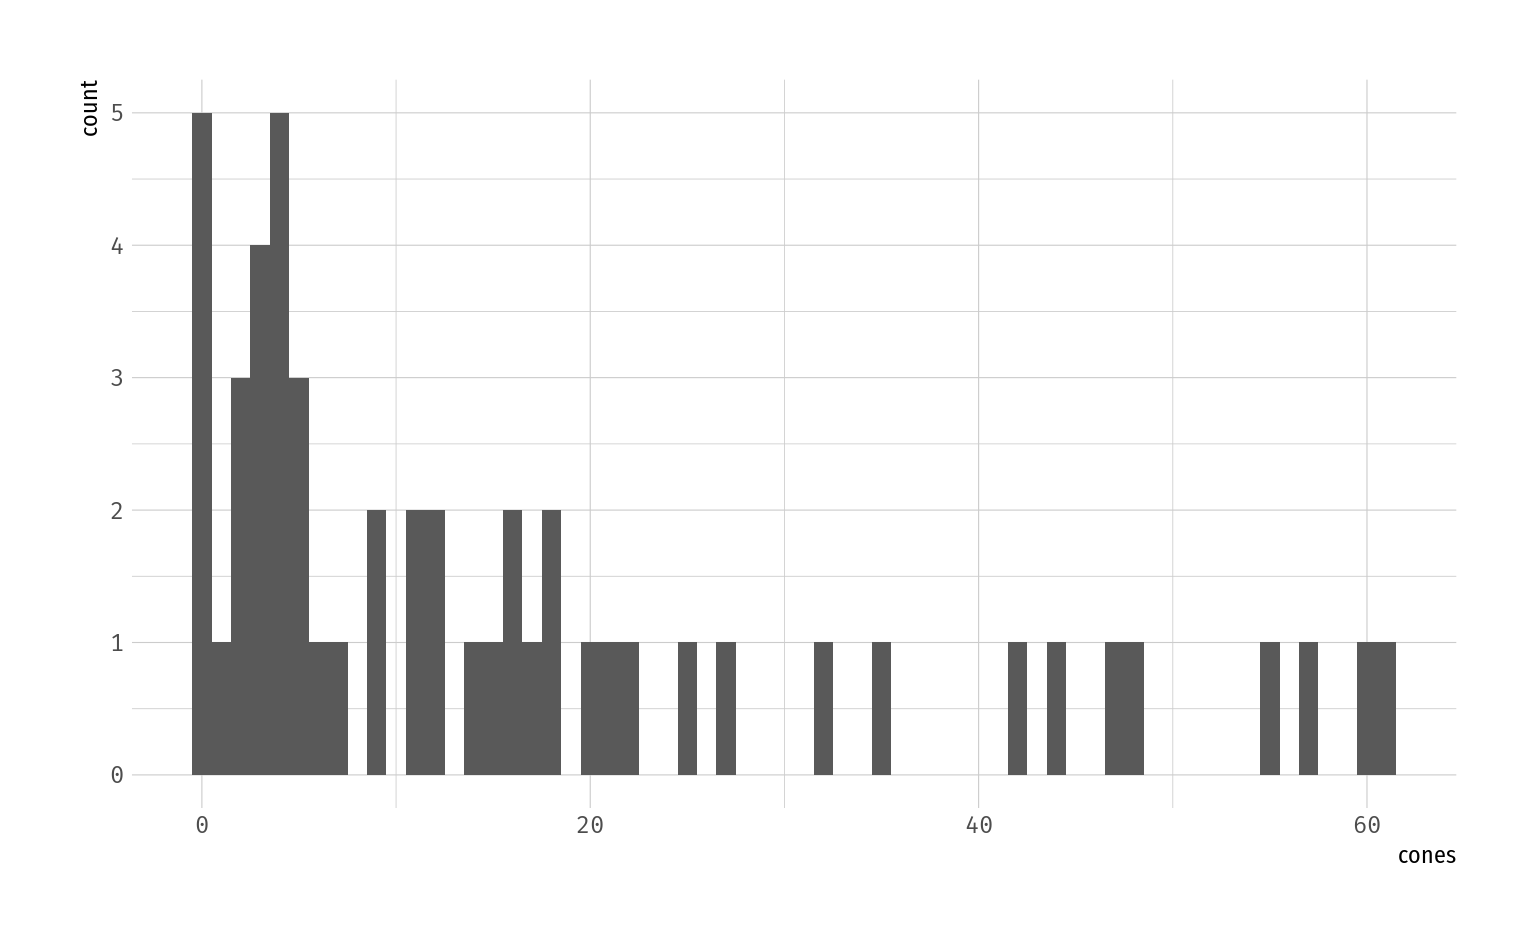
\includegraphics{poisson-regression_files/figure-latex/nbh-1} \end{center}

\begin{Shaded}
\begin{Highlighting}[]
\CommentTok{# Poisson-Modell als Startpunkt}
\NormalTok{m_pois <-}\StringTok{ }\KeywordTok{glm}\NormalTok{(cones }\OperatorTok{~}\StringTok{ }\NormalTok{sntrees }\OperatorTok{+}\StringTok{ }\NormalTok{sheight }\OperatorTok{+}\StringTok{ }\NormalTok{scover, }\DataTypeTok{family =} \KeywordTok{poisson}\NormalTok{(), }\DataTypeTok{data =}\NormalTok{ nuts) }
\KeywordTok{dispersion}\NormalTok{(m_pois) }\CommentTok{# -> overdispersion }
\end{Highlighting}
\end{Shaded}

\begin{verbatim}
#> X-squared(47) = 643.01
#> Pearson Dispersion = 13.681
\end{verbatim}

\begin{Shaded}
\begin{Highlighting}[]
\CommentTok{# NB-Modell}
\NormalTok{m_nb <-}\StringTok{ }\NormalTok{msme}\OperatorTok{::}\KeywordTok{nbinomial}\NormalTok{(cones }\OperatorTok{~}\StringTok{ }\NormalTok{sntrees }\OperatorTok{+}\StringTok{ }\NormalTok{sheight }\OperatorTok{+}\StringTok{ }\NormalTok{scover, }\DataTypeTok{data =}\NormalTok{ nuts)}
\KeywordTok{summary}\NormalTok{(m_nb) }\CommentTok{# Dispersion < 1 -> NB-underdispersed}
\end{Highlighting}
\end{Shaded}

\begin{verbatim}
#> 
#> Call:
#> ml_glm2(formula1 = formula1, formula2 = formula2, data = data, 
#>     family = family, mean.link = mean.link, scale.link = scale.link, 
#>     offset = offset, start = start, verbose = verbose)
#> 
#> Deviance Residuals:
#>    Min. 1st Qu.  Median    Mean 3rd Qu.    Max. 
#> -2.4506 -1.0501 -0.4199 -0.3294  0.3910  1.6464 
#> 
#> Pearson Residuals:
#>       Min.    1st Qu.     Median       Mean    3rd Qu.       Max. 
#> -1.0061432 -0.7292929 -0.3653465  0.0003247  0.4433920  2.6100790 
#> 
#> Coefficients (all in linear predictor):
#>               Estimate    SE     Z        p      LCL   UCL
#> (Intercept)      2.627 0.142 18.53 1.24e-76  2.34948 2.905
#> sntrees          0.306 0.161  1.90   0.0573 -0.00945 0.621
#> sheight          0.158 0.159  0.99    0.322 -0.15463 0.470
#> scover           0.536 0.179  3.00  0.00274  0.18516 0.886
#> (Intercept)_s    0.927 0.199  4.65 3.37e-06  0.53584 1.318
#> 
#> Null deviance: 77.26177  on  49 d.f.
#> Residual deviance: 59.07252  on  46 d.f.
#> Null Pearson: 58.54636  on  49 d.f.
#> Residual Pearson: 41.19523  on  46 d.f.
#> Dispersion: 0.8955486
#> AIC:  383.8132
#> 
#> Number of optimizer iterations:  53
\end{verbatim}

\begin{Shaded}
\begin{Highlighting}[]
\CommentTok{# NB-H: Ursache der Dispersion?}
\NormalTok{m_nbh <-}\StringTok{ }\NormalTok{msme}\OperatorTok{::}\KeywordTok{nbinomial}\NormalTok{(cones }\OperatorTok{~}\StringTok{ }\NormalTok{sntrees }\OperatorTok{+}\StringTok{ }\NormalTok{sheight }\OperatorTok{+}\StringTok{ }\NormalTok{scover, }
                         \DataTypeTok{formula2 =}\NormalTok{ cones }\OperatorTok{~}\StringTok{ }\NormalTok{sntrees }\OperatorTok{+}\StringTok{ }\NormalTok{sheight }\OperatorTok{+}\StringTok{ }\NormalTok{scover,}
                         \DataTypeTok{scale.link =} \StringTok{"log_s"}\NormalTok{,}
                         \DataTypeTok{family =} \StringTok{"negBinomial"}\NormalTok{,}
                         \DataTypeTok{data =}\NormalTok{ nuts)}
\KeywordTok{summary}\NormalTok{(m_nbh)}
\end{Highlighting}
\end{Shaded}

\begin{verbatim}
#> 
#> Call:
#> ml_glm2(formula1 = formula1, formula2 = formula2, data = data, 
#>     family = family, mean.link = mean.link, scale.link = scale.link, 
#>     offset = offset, start = start, verbose = verbose)
#> 
#> Deviance Residuals:
#>    Min. 1st Qu.  Median    Mean 3rd Qu.    Max. 
#> -2.7908 -0.9137 -0.3023 -0.3208  0.4419  1.5671 
#> 
#> Pearson Residuals:
#>     Min.  1st Qu.   Median     Mean  3rd Qu.     Max. 
#> -1.14680 -0.70958 -0.23947  0.03088  0.31546  3.20165 
#> 
#> Coefficients (all in linear predictor):
#>               Estimate    SE      Z        p     LCL   UCL
#> (Intercept)     2.6147 0.144 18.159  1.1e-73  2.3325 2.897
#> sntrees         0.2731 0.110  2.478   0.0132  0.0571 0.489
#> sheight         0.0744 0.144  0.516    0.606 -0.2081 0.357
#> scover          0.5217 0.158  3.300 0.000967  0.2118 0.832
#> (Intercept)_s  -0.1950 0.238 -0.821    0.412 -0.6608 0.271
#> sntrees_s      -0.3834 0.323 -1.186    0.236 -1.0168 0.250
#> sheight_s       0.3312 0.321  1.033    0.302 -0.2973 0.960
#> scover_s        0.2723 0.417  0.652    0.514 -0.5459 1.091
#> 
#> Null deviance: 85.07187  on  49 d.f.
#> Residual deviance: 59.49816  on  43 d.f.
#> Null Pearson: 45.30266  on  49 d.f.
#> Residual Pearson: 46.82167  on  43 d.f.
#> Dispersion: 1.088876
#> AIC:  385.7116
#> 
#> Number of optimizer iterations:  54
\end{verbatim}

Signifikanz der Dispersionsprädiktoren (Suffix \texttt{\_s}) kann nun verwendet werden, um Ursachen der overdispersion zu identifizieren -- auch wenn in diesem Beispiel keiner der Koeffizienten signifikant wird.

\hypertarget{mod-nbp}{%
\subsubsection{Negative binomial-P (NB-P)}\label{mod-nbp}}

Eine Erweiterung der NB1 und NB2, die den Exponenten im Varianzterm parametrisiert (\(\rho\)), womit die Dispersion nun nicht mehr statisch für alle Beobachtungen ist:

\BeginKnitrBlock{definition}[NB-P]
\protect\hypertarget{def:defnbp}{}{\label{def:defnbp} \iffalse (NB-P) \fi{} }\begin{align*}
  \text{NB-P: }\qquad \mathrm{Var}(Y) &= \mu + \alpha\mu^\rho \\
  \text{NB1: } \qquad \mathrm{Var}(Y) &= \mu + \alpha\mu      \\
  \text{NB2: } \qquad \mathrm{Var}(Y) &= \mu + \alpha\mu^2
\end{align*}
\EndKnitrBlock{definition}

Damit ist NB-P äquivalent zu NB2 für \(\rho = 2\) bzw. NB1 für \(\rho = 1\).\\
Um zu evaluieren, ob ein NB1 oder NB2 Modell einen besseren Fit liefert, kann man nun ein NB-P Modell zum Vergleich fitten und Likelihood Ratio Tests zum Vergleich heranziehen.

Siehe auch \citet{hilbeModelingCountData2014} (p.~155) -- wo der Autor zwar den obigen Ansatz beschreibt, aber zur Entscheidung zwischen NB1/2 zusätzlich auf die sowieso etablierten Informationskriteren (AIC/BIC) zurückgreift. Dazu gehört auch, dass das NB-P kein rein diagnostisches Werkzeug sein muss: Wenn ein NB-P ein \emph{deutlich} kleineres AIC aufweist als NB1/2-Modelle, kann das NB-P auch als Modell der Wahl in Erwägung gezogen werden.

\hypertarget{mod-zi}{%
\subsection{\texorpdfstring{Zero-Inflated Models (\emph{mixture models})}{Zero-Inflated Models (mixture models)}}\label{mod-zi}}

Zero-inflated Modelle sind \emph{mixtures}, das heißt, sie entstehen durch Mischung zweier Wahrscheinlichkeitsfunktionen. In der Regel wird eine Nullverteilung mit einer regulären Zählverteilung (Poisson, NB, PIG, \ldots{}) \enquote{gemischt}, abhängig von einem \emph{mixture parameter} \(\pi \in [0,1]\), der z.B. logistisch modelliert wird. Die Nullen im Modell werden dementsprechend durch beide Verteilungen (Nullverteilung, Zählverteilung) beschrieben -- im Gegensatz zu \emph{hurdle models} (vgl. \ref{mod-hurdle}), die Nullen logistisch und die positiven counts über eine \emph{truncated} distribution modellieren würden.

Zero-inflated distributions wie ZIP und ZINB wurden hergeleitet als zweiteilige mixture distributions. Die allgemeine Form für mixture distributions ist

\BeginKnitrBlock{definition}[Mixture distribution und zero-inflated distribution]
\protect\hypertarget{def:defmixture}{}{\label{def:defmixture} \iffalse (Mixture distribution und zero-inflated distribution) \fi{} }\begin{equation*}
  P(Y = y) = p \cdot g_1(y) + (1-p) \cdot g_2(y)
\end{equation*}

mit \(p\) als \emph{mixture proportion} und \(g_1, g_2\) als Dichte-/Massefunktionen der beiden Komponenten.

Für zero-inflation setzt man \(p\) als \emph{rate of zero-inflation} \(\pi\), \(g_1\) als degenerierten 0-Verteilung und \(g_2\) als Poisson-PMF oder ähnliche Zähl-Verteilung wie NB, PIG, etc.

Eine alternative Darstellung für eine \emph{zero-inflated} Verteilung (\href{https://www.statistik.uni-dortmund.de/useR-2008/slides/Kleiber+Zeileis.pdf}{siehe}):

\begin{equation*}
f_\mathrm{zeroinfl} (y; x, \beta, \pi) = \pi \cdot I_{\{0\}}(y) + (1 - \pi) \cdot f_{\mathrm{count}}(y; x, \beta)
\end{equation*}

Mit zu modellierendem Erwartungswert

\begin{equation*}
\mu_i = \pi_i \cdot 0 + (1 - \pi_i) \cdot \exp(x_i^T\beta)
\end{equation*}

Wobei \(\pi\) in der Regel binomial, bzw. mittels logistischer Regression geschätzt wird.
\EndKnitrBlock{definition}

\BeginKnitrBlock{definition}[Zero-Inflated Poisson Verteilung (ZIP)]
\protect\hypertarget{def:defzip}{}{\label{def:defzip} \iffalse (Zero-Inflated Poisson Verteilung (ZIP)) \fi{} }Nach \citet{perumean-chaneyZeroinflatedOverdispersedWhat2013} (p.~1675)

\begin{align*}
P(Y = 0) &= \pi + (1-\pi) \cdot e^{-\mu} \\
P(Y = y) &= (1 - \pi) \cdot \frac{\mu^y e^{-\mu}}{y!}, \quad y = 1, 2, 3, \ldots
\end{align*}
\EndKnitrBlock{definition}

\BeginKnitrBlock{definition}[Zero-Inflated Negative Binomialverteilung (ZINB)]
\protect\hypertarget{def:defzinb}{}{\label{def:defzinb} \iffalse (Zero-Inflated Negative Binomialverteilung (ZINB)) \fi{} }Nach \citet{perumean-chaneyZeroinflatedOverdispersedWhat2013} (p.~1675)

\begin{align*}
P(Y = 0) &= \pi + (1 - \pi) \cdot \frac{\theta^\theta}{(\theta + \mu)^\theta}  \\
P(Y = y) &= (1 - \pi) \cdot \frac{\Gamma(\theta+y)}{\Gamma(\theta) \Gamma(y + 1)} \frac{\theta^\theta \mu^y}{(\theta + \mu)^{(\theta + y)}}, \quad y = 1, 2, 3, \ldots
\end{align*}
\EndKnitrBlock{definition}

\hypertarget{anwendung}{%
\section{Anwendung}\label{anwendung}}

Als Beispiel verwenden wir hier \texttt{rwm1984}, ein Subset des Datensatz \texttt{rwm5yr} (vgl. Abschnitt \ref{data}, \texttt{?COUNT::rwm1984}), der Angaben zur Anzahl der Arztbesuche pro Person mit zusätzlichen demographischen Merkmalen enthält. Für unser Beispielmodell verwenden wir folgende Variablen:

\begin{itemize}
\tightlist
\item
  \texttt{docvis}: Abhängige Variable, Anzahl der Arztbesuche im Jahr (0-121)
\item
  \texttt{outwork}: Arbeitslos (1), arbeitend (0)
\item
  \texttt{age}: Alter (25 - 64)
\end{itemize}

\begin{Shaded}
\begin{Highlighting}[]
\CommentTok{# Daten (bemerke: rwm1984 ist kein exportiertes Objekt in COUNT)}
\KeywordTok{data}\NormalTok{(rwm1984, }\DataTypeTok{package =} \StringTok{"COUNT"}\NormalTok{)}

\CommentTok{# Model fit}
\NormalTok{mod_rwm <-}\StringTok{ }\KeywordTok{glm}\NormalTok{(docvis }\OperatorTok{~}\StringTok{ }\NormalTok{outwork }\OperatorTok{+}\StringTok{ }\NormalTok{age, }\DataTypeTok{family =} \KeywordTok{poisson}\NormalTok{(), }\DataTypeTok{data =}\NormalTok{ rwm1984)}

\CommentTok{# Summary display}
\KeywordTok{pander}\NormalTok{(mod_rwm)}
\end{Highlighting}
\end{Shaded}

\begin{longtable}[]{@{}ccccc@{}}
\caption{Fitting generalized (poisson/log) linear model: docvis \textasciitilde{} outwork + age}\tabularnewline
\toprule
\begin{minipage}[b]{0.21\columnwidth}\centering
~\strut
\end{minipage} & \begin{minipage}[b]{0.13\columnwidth}\centering
Estimate\strut
\end{minipage} & \begin{minipage}[b]{0.16\columnwidth}\centering
Std. Error\strut
\end{minipage} & \begin{minipage}[b]{0.12\columnwidth}\centering
z value\strut
\end{minipage} & \begin{minipage}[b]{0.16\columnwidth}\centering
Pr(\textgreater{}\textbar{}z\textbar{})\strut
\end{minipage}\tabularnewline
\midrule
\endfirsthead
\toprule
\begin{minipage}[b]{0.21\columnwidth}\centering
~\strut
\end{minipage} & \begin{minipage}[b]{0.13\columnwidth}\centering
Estimate\strut
\end{minipage} & \begin{minipage}[b]{0.16\columnwidth}\centering
Std. Error\strut
\end{minipage} & \begin{minipage}[b]{0.12\columnwidth}\centering
z value\strut
\end{minipage} & \begin{minipage}[b]{0.16\columnwidth}\centering
Pr(\textgreater{}\textbar{}z\textbar{})\strut
\end{minipage}\tabularnewline
\midrule
\endhead
\begin{minipage}[t]{0.21\columnwidth}\centering
\textbf{(Intercept)}\strut
\end{minipage} & \begin{minipage}[t]{0.13\columnwidth}\centering
-0.03352\strut
\end{minipage} & \begin{minipage}[t]{0.16\columnwidth}\centering
0.03918\strut
\end{minipage} & \begin{minipage}[t]{0.12\columnwidth}\centering
-0.8554\strut
\end{minipage} & \begin{minipage}[t]{0.16\columnwidth}\centering
0.3923\strut
\end{minipage}\tabularnewline
\begin{minipage}[t]{0.21\columnwidth}\centering
\textbf{outwork}\strut
\end{minipage} & \begin{minipage}[t]{0.13\columnwidth}\centering
0.4079\strut
\end{minipage} & \begin{minipage}[t]{0.16\columnwidth}\centering
0.01884\strut
\end{minipage} & \begin{minipage}[t]{0.12\columnwidth}\centering
21.65\strut
\end{minipage} & \begin{minipage}[t]{0.16\columnwidth}\centering
6.481e-104\strut
\end{minipage}\tabularnewline
\begin{minipage}[t]{0.21\columnwidth}\centering
\textbf{age}\strut
\end{minipage} & \begin{minipage}[t]{0.13\columnwidth}\centering
0.02208\strut
\end{minipage} & \begin{minipage}[t]{0.16\columnwidth}\centering
0.0008377\strut
\end{minipage} & \begin{minipage}[t]{0.12\columnwidth}\centering
26.36\strut
\end{minipage} & \begin{minipage}[t]{0.16\columnwidth}\centering
3.73e-153\strut
\end{minipage}\tabularnewline
\bottomrule
\end{longtable}

\begin{Shaded}
\begin{Highlighting}[]
\KeywordTok{pander}\NormalTok{(}\KeywordTok{glance}\NormalTok{(mod_rwm))}
\end{Highlighting}
\end{Shaded}

\begin{longtable}[]{@{}ccccccc@{}}
\toprule
\begin{minipage}[b]{0.17\columnwidth}\centering
null.deviance\strut
\end{minipage} & \begin{minipage}[b]{0.11\columnwidth}\centering
df.null\strut
\end{minipage} & \begin{minipage}[b]{0.10\columnwidth}\centering
logLik\strut
\end{minipage} & \begin{minipage}[b]{0.09\columnwidth}\centering
AIC\strut
\end{minipage} & \begin{minipage}[b]{0.09\columnwidth}\centering
BIC\strut
\end{minipage} & \begin{minipage}[b]{0.12\columnwidth}\centering
deviance\strut
\end{minipage} & \begin{minipage}[b]{0.15\columnwidth}\centering
df.residual\strut
\end{minipage}\tabularnewline
\midrule
\endhead
\begin{minipage}[t]{0.17\columnwidth}\centering
25791\strut
\end{minipage} & \begin{minipage}[t]{0.11\columnwidth}\centering
3873\strut
\end{minipage} & \begin{minipage}[t]{0.10\columnwidth}\centering
-15636\strut
\end{minipage} & \begin{minipage}[t]{0.09\columnwidth}\centering
31279\strut
\end{minipage} & \begin{minipage}[t]{0.09\columnwidth}\centering
31298\strut
\end{minipage} & \begin{minipage}[t]{0.12\columnwidth}\centering
24190\strut
\end{minipage} & \begin{minipage}[t]{0.15\columnwidth}\centering
3871\strut
\end{minipage}\tabularnewline
\bottomrule
\end{longtable}

Das erste was wir zur Evaluation unseres Modells tun können, ohne direkt andere Modelle zum vergleich heranzuziehen, ist die beobachteten Counts und die auf Basis des Modells erwarteten Counts zu vergleichen, um ein grobes Gefühl für die Situation zu erhalten (Code frei adaptiert nach \citet{hilbeModelingCountData2014}, p.~88f):

\begin{Shaded}
\begin{Highlighting}[]
\CommentTok{# Beobachtete und erwartete counts}
\NormalTok{observed_v_expected <-}\StringTok{ }\NormalTok{rwm1984 }\OperatorTok
\StringTok{  }\KeywordTok{count}\NormalTok{(docvis, }\DataTypeTok{name =} \StringTok{"observed"}\NormalTok{) }\OperatorTok
\StringTok{  }\KeywordTok{mutate}\NormalTok{(}
    \DataTypeTok{expected =}\NormalTok{ purrr}\OperatorTok{::}\KeywordTok{map_dbl}\NormalTok{(docvis, }\OperatorTok{~}\NormalTok{\{}
                  \KeywordTok{dpois}\NormalTok{(.x, }\KeywordTok{fitted}\NormalTok{(mod)) }\OperatorTok
\StringTok{                    }\KeywordTok{sum}\NormalTok{() }\OperatorTok
\StringTok{                    }\KeywordTok{round}\NormalTok{(}\DecValTok{2}\NormalTok{)}
\NormalTok{                \}),}
    \DataTypeTok{difference =}\NormalTok{ observed }\OperatorTok{-}\StringTok{ }\NormalTok{expected}
\NormalTok{  ) }

\NormalTok{observed_v_expected }\OperatorTok
\StringTok{  }\KeywordTok{head}\NormalTok{(}\DecValTok{5}\NormalTok{) }\OperatorTok
\StringTok{  }\KeywordTok{pander}\NormalTok{(}\DataTypeTok{caption =} \StringTok{"Observed and expected counts"}\NormalTok{)}
\end{Highlighting}
\end{Shaded}

\begin{longtable}[]{@{}cccc@{}}
\caption{Observed and expected counts}\tabularnewline
\toprule
\begin{minipage}[b]{0.11\columnwidth}\centering
docvis\strut
\end{minipage} & \begin{minipage}[b]{0.14\columnwidth}\centering
observed\strut
\end{minipage} & \begin{minipage}[b]{0.14\columnwidth}\centering
expected\strut
\end{minipage} & \begin{minipage}[b]{0.16\columnwidth}\centering
difference\strut
\end{minipage}\tabularnewline
\midrule
\endfirsthead
\toprule
\begin{minipage}[b]{0.11\columnwidth}\centering
docvis\strut
\end{minipage} & \begin{minipage}[b]{0.14\columnwidth}\centering
observed\strut
\end{minipage} & \begin{minipage}[b]{0.14\columnwidth}\centering
expected\strut
\end{minipage} & \begin{minipage}[b]{0.16\columnwidth}\centering
difference\strut
\end{minipage}\tabularnewline
\midrule
\endhead
\begin{minipage}[t]{0.11\columnwidth}\centering
0\strut
\end{minipage} & \begin{minipage}[t]{0.14\columnwidth}\centering
1611\strut
\end{minipage} & \begin{minipage}[t]{0.14\columnwidth}\centering
106.2\strut
\end{minipage} & \begin{minipage}[t]{0.16\columnwidth}\centering
1505\strut
\end{minipage}\tabularnewline
\begin{minipage}[t]{0.11\columnwidth}\centering
1\strut
\end{minipage} & \begin{minipage}[t]{0.14\columnwidth}\centering
448\strut
\end{minipage} & \begin{minipage}[t]{0.14\columnwidth}\centering
194.1\strut
\end{minipage} & \begin{minipage}[t]{0.16\columnwidth}\centering
253.9\strut
\end{minipage}\tabularnewline
\begin{minipage}[t]{0.11\columnwidth}\centering
2\strut
\end{minipage} & \begin{minipage}[t]{0.14\columnwidth}\centering
440\strut
\end{minipage} & \begin{minipage}[t]{0.14\columnwidth}\centering
186.8\strut
\end{minipage} & \begin{minipage}[t]{0.16\columnwidth}\centering
253.2\strut
\end{minipage}\tabularnewline
\begin{minipage}[t]{0.11\columnwidth}\centering
3\strut
\end{minipage} & \begin{minipage}[t]{0.14\columnwidth}\centering
353\strut
\end{minipage} & \begin{minipage}[t]{0.14\columnwidth}\centering
129.9\strut
\end{minipage} & \begin{minipage}[t]{0.16\columnwidth}\centering
223.1\strut
\end{minipage}\tabularnewline
\begin{minipage}[t]{0.11\columnwidth}\centering
4\strut
\end{minipage} & \begin{minipage}[t]{0.14\columnwidth}\centering
213\strut
\end{minipage} & \begin{minipage}[t]{0.14\columnwidth}\centering
76.99\strut
\end{minipage} & \begin{minipage}[t]{0.16\columnwidth}\centering
136\strut
\end{minipage}\tabularnewline
\bottomrule
\end{longtable}

\begin{Shaded}
\begin{Highlighting}[]
\CommentTok{# Mittelwert und Varianz der jeweiligen counts}
\CommentTok{# (für "expected" gilt Varianz := Mittelwert)}
\KeywordTok{tribble}\NormalTok{(}
  \OperatorTok{~}\NormalTok{Counts,   }\OperatorTok{~}\NormalTok{Mean,                 }\OperatorTok{~}\NormalTok{Variance,}
  \StringTok{"observed"}\NormalTok{, }\KeywordTok{mean}\NormalTok{(rwm1984}\OperatorTok{$}\NormalTok{docvis), }\KeywordTok{var}\NormalTok{(rwm1984}\OperatorTok{$}\NormalTok{docvis),}
  \StringTok{"expected"}\NormalTok{, }\KeywordTok{mean}\NormalTok{(}\KeywordTok{fitted}\NormalTok{(mod)),    }\KeywordTok{mean}\NormalTok{(}\KeywordTok{fitted}\NormalTok{(mod))}
\NormalTok{) }\OperatorTok
\StringTok{  }\KeywordTok{pander}\NormalTok{(}\DataTypeTok{caption =} \StringTok{"Mean & variance of observed and expected counts"}\NormalTok{)}
\end{Highlighting}
\end{Shaded}

\begin{longtable}[]{@{}ccc@{}}
\caption{Mean \& variance of observed and expected counts}\tabularnewline
\toprule
\begin{minipage}[b]{0.14\columnwidth}\centering
Counts\strut
\end{minipage} & \begin{minipage}[b]{0.10\columnwidth}\centering
Mean\strut
\end{minipage} & \begin{minipage}[b]{0.14\columnwidth}\centering
Variance\strut
\end{minipage}\tabularnewline
\midrule
\endfirsthead
\toprule
\begin{minipage}[b]{0.14\columnwidth}\centering
Counts\strut
\end{minipage} & \begin{minipage}[b]{0.10\columnwidth}\centering
Mean\strut
\end{minipage} & \begin{minipage}[b]{0.14\columnwidth}\centering
Variance\strut
\end{minipage}\tabularnewline
\midrule
\endhead
\begin{minipage}[t]{0.14\columnwidth}\centering
observed\strut
\end{minipage} & \begin{minipage}[t]{0.10\columnwidth}\centering
3.163\strut
\end{minipage} & \begin{minipage}[t]{0.14\columnwidth}\centering
39.39\strut
\end{minipage}\tabularnewline
\begin{minipage}[t]{0.14\columnwidth}\centering
expected\strut
\end{minipage} & \begin{minipage}[t]{0.10\columnwidth}\centering
5.401\strut
\end{minipage} & \begin{minipage}[t]{0.14\columnwidth}\centering
5.401\strut
\end{minipage}\tabularnewline
\bottomrule
\end{longtable}

\begin{Shaded}
\begin{Highlighting}[]
\CommentTok{# Plot: observed vs. expected counts}
\NormalTok{observed_v_expected }\OperatorTok
\StringTok{  }\KeywordTok{filter}\NormalTok{(docvis }\OperatorTok{<=}\StringTok{ }\DecValTok{12}\NormalTok{) }\OperatorTok
\StringTok{  }\KeywordTok{gather}\NormalTok{(type, count, observed, expected) }\OperatorTok
\StringTok{  }\KeywordTok{ggplot}\NormalTok{(}\KeywordTok{aes}\NormalTok{(}\DataTypeTok{x =}\NormalTok{ docvis, }\DataTypeTok{y =}\NormalTok{ count, }\DataTypeTok{fill =}\NormalTok{ type, }\DataTypeTok{color =}\NormalTok{ type)) }\OperatorTok{+}
\StringTok{  }\KeywordTok{geom_point}\NormalTok{(}\DataTypeTok{shape =} \DecValTok{21}\NormalTok{, }\DataTypeTok{color =} \StringTok{"black"}\NormalTok{, }\DataTypeTok{stroke =} \FloatTok{.5}\NormalTok{, }\DataTypeTok{size =} \DecValTok{2}\NormalTok{) }\OperatorTok{+}
\StringTok{  }\KeywordTok{geom_path}\NormalTok{(}\DataTypeTok{linetype =} \StringTok{"dotted"}\NormalTok{, }\DataTypeTok{size =} \FloatTok{.25}\NormalTok{) }\OperatorTok{+}
\StringTok{  }\KeywordTok{scale_x_continuous}\NormalTok{(}\DataTypeTok{breaks =} \KeywordTok{seq}\NormalTok{(}\DecValTok{0}\NormalTok{, }\DecValTok{12}\NormalTok{, }\DecValTok{2}\NormalTok{)) }\OperatorTok{+}
\StringTok{  }\KeywordTok{scale_fill_brewer}\NormalTok{(}\DataTypeTok{palette =} \StringTok{"Set1"}\NormalTok{, }\DataTypeTok{aesthetics =} \KeywordTok{c}\NormalTok{(}\StringTok{"color"}\NormalTok{, }\StringTok{"fill"}\NormalTok{), }\DataTypeTok{name =} \StringTok{""}\NormalTok{) }\OperatorTok{+}
\StringTok{  }\KeywordTok{labs}\NormalTok{(}
    \DataTypeTok{title =} \StringTok{"rwm1984: Poisson Modell"}\NormalTok{,}
    \DataTypeTok{subtitle =} \StringTok{"Observed und expected counts bei overdispersion"}\NormalTok{,}
    \DataTypeTok{caption =} \StringTok{"Output begrenzt auf docvs <= 12"}\NormalTok{,}
    \DataTypeTok{x =} \StringTok{"Anzahl der Arztbesuche (docvis)"}\NormalTok{, }\DataTypeTok{y =} \StringTok{"Count"}
\NormalTok{  ) }\OperatorTok{+}
\StringTok{  }\KeywordTok{theme}\NormalTok{(}\DataTypeTok{legend.position =} \StringTok{"top"}\NormalTok{)}
\end{Highlighting}
\end{Shaded}

\begin{center}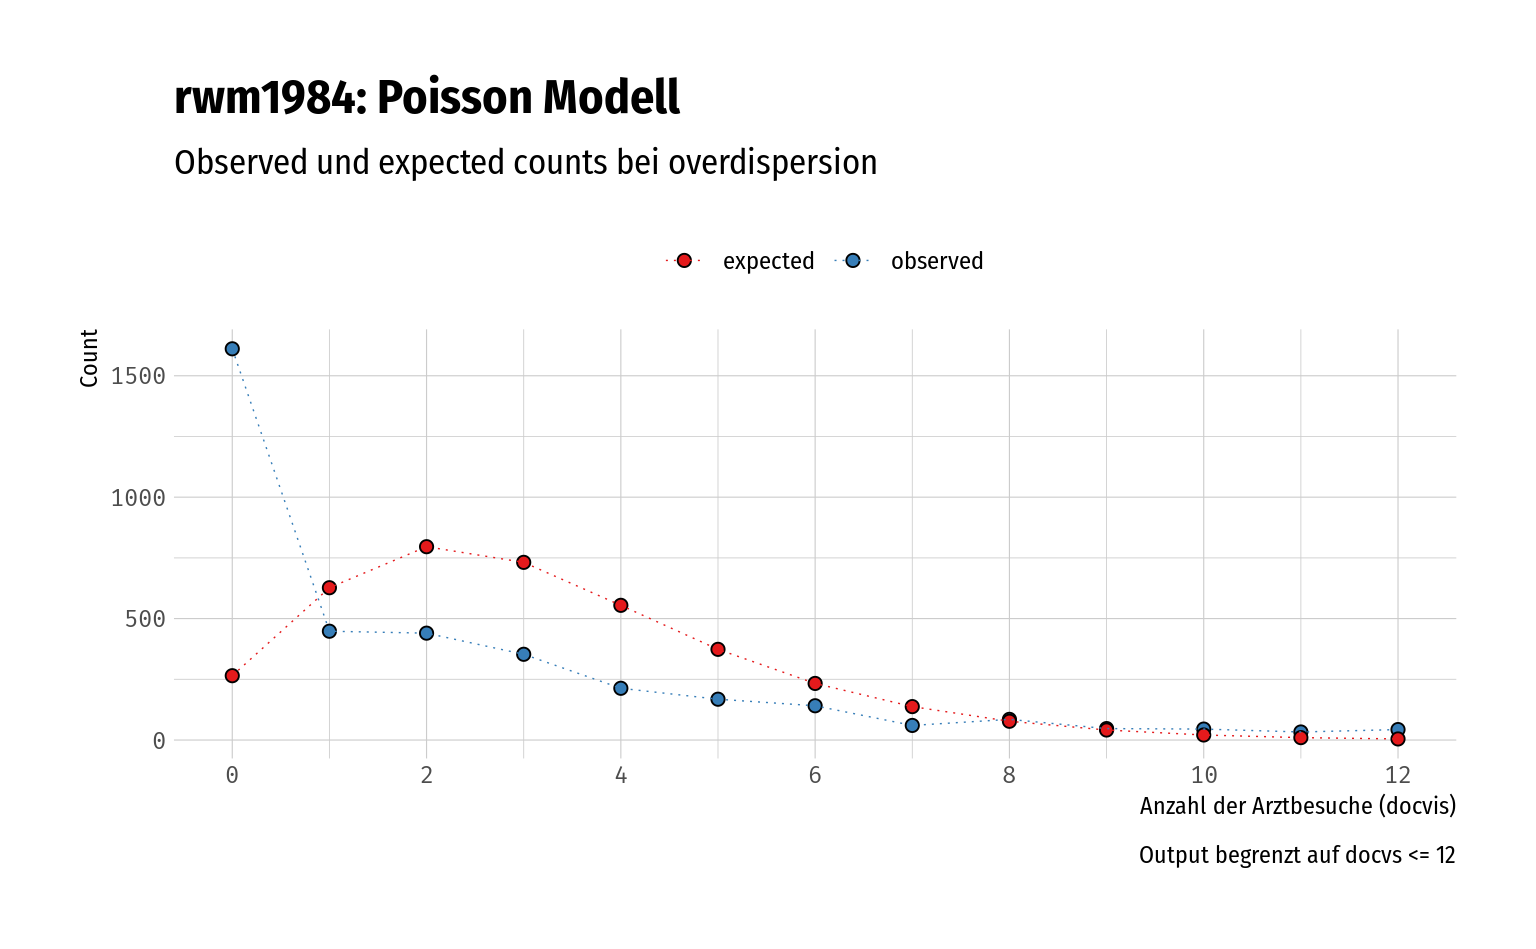
\includegraphics{poisson-regression_files/figure-latex/diag_compare_expected-1} \end{center}

Anhand der ersten Tabelle können wir recht schnell erkennen, dass wir hier \emph{deutlich} mehr Nullen beobachten als das Modell vorhersagt -- mehr dazu in Abschnitt \ref{zeros}.\\
Der Plot veranschaulicht den eher suboptimalen model fit unter diesen Umständen (overdispersion \& zero-inflation).

\hypertarget{overdisp-diag}{%
\subsection{Overdispersion: Erkennung und Handhabung}\label{overdisp-diag}}

Der \emph{Score-Test} wird nicht unbedingt empfohlen, findet sich aber in der Literatur:

\BeginKnitrBlock{definition}[Score-Test auf Overdispersion]
\protect\hypertarget{def:unnamed-chunk-3}{}{\label{def:unnamed-chunk-3} \iffalse (Score-Test auf Overdispersion) \fi{} }Nach \citet{hilbeModelingCountData2014} (p.~85f):

Sei \(Y\) die abhängige Variable und \(y_i\) die \(i-te\) Beobachtung, mit \(\hat{\mu}_i\) als gefitteter Wert eines Poisson-Modells, dann wird der z-Score wie folgt berechnet:

\begin{equation}
  z_i = \frac{(y_i - \hat{\mu})^2 -y}{\hat{\mu} \sqrt{2}}
\end{equation}

Zur Evaluation von \(z\) wird z.B. ein Intercept-only Regressionsmodell mit \(z\) als abhängiger Variable gefitted, mit der Nullhypothese \enquote{Es liegt keine Overdispersion vor}.

Dabei gelten folgende Annahmen:

\begin{enumerate}
\def\labelenumi{\arabic{enumi}.}
\tightlist
\item
  Die Stichprobe ist \emph{groß}
\item
  \(z\) ist t-verteilt
\end{enumerate}
\EndKnitrBlock{definition}

\BeginKnitrBlock{definition}[Lagrange Multiplier Test]
\protect\hypertarget{def:unnamed-chunk-4}{}{\label{def:unnamed-chunk-4} \iffalse (Lagrange Multiplier Test) \fi{} }Nach \citet{hilbeModelingCountData2014} (p.~85f):

Eine \(\chi^2\)-Teststatistik mit einem Freiheitsgrad.

\begin{equation}
  \chi^2 = \frac{\left( \sum_{i=1}^n \hat{\mu}_i^2 - n \bar{y} \right)^2}
                {2 \sum_{i=1}^n \hat{\mu}_i^2}
\end{equation}
\EndKnitrBlock{definition}

Eine rudimentäre R-Implementation findet sich in Abschnitt \ref{helperfuns}.

\hypertarget{boundary-likelihood-ratio-test-blr}{%
\subsubsection{(Boundary) Likelihood Ratio Test (BLR)}\label{boundary-likelihood-ratio-test-blr}}

Zum vergleich von zwei geschachtelten (\emph{nested}) Modellen kann der \emph{Likelihood Ratio Test} verwendet werden:

\BeginKnitrBlock{definition}[Likelihood Ratio Test]
\protect\hypertarget{def:LRT}{}{\label{def:LRT} \iffalse (Likelihood Ratio Test) \fi{} }\begin{equation}
 LR = -2 (\mathcal{L}_R - \mathcal{L}_F)
\end{equation}

Mit \(\mathcal{L}_F\) als log-likelihood des vollen (oder \enquote{größeren}) Modells, und \(\mathcal{L}_R\) als log-likelihood des reduzierteren Modells.
\EndKnitrBlock{definition}

Eine Variante des Tests kann verwendet werden, um den Dispersionsparameter \(\alpha\) eines NB-Modells zu testen. Da eine NB-Verteilung für \(\alpha = 0\) äquivalent zur Poisson ist (siehe Abschnitt \ref{mod-nb}), kann ein Poisson-Modell als reduzierte Variante eines NB-Modells betrachtet werden. In diesem Fall verwendet man den \emph{Boundary Likelhihood Ratio} test:

\BeginKnitrBlock{definition}[Boundary Likelihood Ratio Test]
\protect\hypertarget{def:BLR}{}{\label{def:BLR} \iffalse (Boundary Likelihood Ratio Test) \fi{} }\begin{equation}
 BLR = -2 (\mathcal{L}_\mathrm{Poisson} - \mathcal{L}_\mathrm{NB})
\end{equation}
\EndKnitrBlock{definition}

\begin{quote}
It is important, though, to remember that the BLR test has a lower limiting case for the value of \(\alpha\), which is what is being tested. Given that the standard parameterization of the negative binomial variance function is \(\mu + \alpha \mu^2\) , when \(\alpha = 0\), the variance reduces to \(\mu\).

--- \citet{hilbeModelingCountData2014}, p.~115
\end{quote}

Der resultierende Wert ist \(\chi^2_{(1)}\)-verteilt. Der resultierende p-Wert muss zusätzlich halbiert werden \citep[siehe][p.~115]{hilbeModelingCountData2014}.

\begin{quote}
Since the distribution being tested can go no lower than 0, that is the boundary. Only one half of the full distribution is used. Therefore the Chi2 (sic!) test is divided by 2

--- \citet{hilbeModelingCountData2014}, p.~115
\end{quote}

Am Beispiel der \texttt{rwm1984}-Daten:

\begin{Shaded}
\begin{Highlighting}[]
\CommentTok{# Poisson-Modell}
\NormalTok{mod_p <-}\StringTok{ }\KeywordTok{glm}\NormalTok{(docvis }\OperatorTok{~}\StringTok{ }\NormalTok{outwork }\OperatorTok{+}\StringTok{ }\NormalTok{age, }\DataTypeTok{family =} \KeywordTok{poisson}\NormalTok{(), }\DataTypeTok{data =}\NormalTok{ rwm1984)}

\CommentTok{# NB-Modell}
\NormalTok{mod_nb <-}\StringTok{ }\NormalTok{MASS}\OperatorTok{::}\KeywordTok{glm.nb}\NormalTok{(docvis }\OperatorTok{~}\StringTok{ }\NormalTok{outwork }\OperatorTok{+}\StringTok{ }\NormalTok{age, }\DataTypeTok{data =}\NormalTok{ rwm1984)}

\CommentTok{# BLR: Recht eindeutig.}
\NormalTok{lmtest}\OperatorTok{::}\KeywordTok{lrtest}\NormalTok{(mod_p, mod_nb)}
\end{Highlighting}
\end{Shaded}

\begin{verbatim}
#> Likelihood ratio test
#> 
#> Model 1: docvis ~ outwork + age
#> Model 2: docvis ~ outwork + age
#>   #Df   LogLik Df Chisq Pr(>Chisq)    
#> 1   3 -15636.4                        
#> 2   4  -8332.8  1 14607  < 2.2e-16 ***
#> ---
#> Signif. codes:  0 '***' 0.001 '**' 0.01 '*' 0.05 '.' 0.1 ' ' 1
\end{verbatim}

\begin{Shaded}
\begin{Highlighting}[]
\CommentTok{# Bei gegebenem BLR-Wert von 4.2 ließe sich der p-Wert wie folgt berechnen:}
\KeywordTok{pchisq}\NormalTok{(}\FloatTok{4.2}\NormalTok{, }\DataTypeTok{df =} \DecValTok{1}\NormalTok{, }\DataTypeTok{lower.tail =} \OtherTok{FALSE}\NormalTok{) }\OperatorTok{/}\StringTok{ }\DecValTok{2}
\end{Highlighting}
\end{Shaded}

\begin{verbatim}
#> [1] 0.02021199
\end{verbatim}

\begin{Shaded}
\begin{Highlighting}[]
\CommentTok{# Oder}
\NormalTok{(}\DecValTok{1} \OperatorTok{-}\StringTok{ }\KeywordTok{pchisq}\NormalTok{(}\FloatTok{4.2}\NormalTok{, }\DataTypeTok{df =} \DecValTok{1}\NormalTok{)) }\OperatorTok{/}\StringTok{ }\DecValTok{2}
\end{Highlighting}
\end{Shaded}

\begin{verbatim}
#> [1] 0.02021199
\end{verbatim}

\hypertarget{umgang-mit-overdispersion}{%
\subsubsection{Umgang mit Overdispersion}\label{umgang-mit-overdispersion}}

Zur expliziten Modellierung des Dispersionparameters kann ein NBH Modell (\ref{mod-nbh}) genutzt werden, falls die Quelle der overdispersion von besonderem Interesse ist.

Abseits davon bleiben 2 grobe Strategien :

\begin{enumerate}
\def\labelenumi{\arabic{enumi}.}
\tightlist
\item
  Adjustierung der durch die overdispersion verzerrten Standardfehler (Quasipoisson, Quasi-Likelihood, robuste Varianzschätzer)
\item
  Wechsel auf ein Modell, das overdispersion (oder allgemeine extradispersion) erlaubt (e.g.~NB)
\end{enumerate}

(Bemerke: Standardfehler für IRRs werden i.A. über die \emph{delta method} bestimmt, die ich noch recherchieren und irgendwo einbauen muss)

\hypertarget{quasipoisson-skalierung-der-standardfehler}{%
\subparagraph{Quasipoisson: Skalierung der Standardfehler}\label{quasipoisson-skalierung-der-standardfehler}}
\addcontentsline{toc}{subparagraph}{Quasipoisson: Skalierung der Standardfehler}

Hier werden lediglich die Standardfehler der Koeffizienten eines Poisson-Modells adjustiert, die bei overdispersion i.d.R. unterschätzt werden -- die eigentliche Parameterschätzung wird nicht beeinflusst:

\[\mathrm{SE}(\beta_k) \cdot \sqrt{D}\]
Wobei \(D\) der Pearson-Dispersionsindex ist (vgl. \citet{hilbeModelingCountData2014}, p.~92ff), den wir in \ref{def:def-pearsondisp} als \(\frac{\chi^2_{\mathrm{Pearson}}}{\mathrm{df}}\) definiert hatten.

Ein möglicher Nachteil jedoch: Es wird zuerst ein reguläres Poisson-Modell gefittet, Standardfehler und Dispersionsindex bestimmt, und dann dasselbe Modell mit skalierten Standardfehlern erneut gefittet -- dementsprechend ist diese Methode vermutlich für größere Datensätze eher ineffizient.

Einmal auf unser voriges Beispiel anhand der \texttt{rwm5yr}-Daten angewandt:

\begin{Shaded}
\begin{Highlighting}[]
\CommentTok{# Urprüngliches Model}
\NormalTok{mod <-}\StringTok{ }\KeywordTok{glm}\NormalTok{(docvis }\OperatorTok{~}\StringTok{ }\NormalTok{outwork }\OperatorTok{+}\StringTok{ }\NormalTok{age, }\DataTypeTok{family =} \KeywordTok{poisson}\NormalTok{(), }\DataTypeTok{data =}\NormalTok{ rwm1984)}

\NormalTok{mod_qp <-}\StringTok{ }\KeywordTok{glm}\NormalTok{(docvis }\OperatorTok{~}\StringTok{ }\NormalTok{outwork }\OperatorTok{+}\StringTok{ }\NormalTok{age, }\DataTypeTok{family =} \KeywordTok{quasipoisson}\NormalTok{(), }\DataTypeTok{data =}\NormalTok{ rwm1984)}

\KeywordTok{dispersion}\NormalTok{(mod)}
\end{Highlighting}
\end{Shaded}

\begin{verbatim}
#> X-squared(3871) = 43909.62
#> Pearson Dispersion = 11.343
\end{verbatim}

\begin{Shaded}
\begin{Highlighting}[]
\KeywordTok{dispersion}\NormalTok{(mod_qp)}
\end{Highlighting}
\end{Shaded}

\begin{verbatim}
#> X-squared(3871) = 43909.62
#> Pearson Dispersion = 11.343
\end{verbatim}

An der Dispersion hat sich nichts geändert, nur an den Standardfehlern der Koeffizienten (in folgenden Tabellen auf log-Skala):

\begin{Shaded}
\begin{Highlighting}[]
\KeywordTok{pander}\NormalTok{(mod, }\DataTypeTok{caption =} \StringTok{"Poisson-Modell"}\NormalTok{)}
\end{Highlighting}
\end{Shaded}

\begin{longtable}[]{@{}ccccc@{}}
\caption{Poisson-Modell}\tabularnewline
\toprule
\begin{minipage}[b]{0.21\columnwidth}\centering
~\strut
\end{minipage} & \begin{minipage}[b]{0.13\columnwidth}\centering
Estimate\strut
\end{minipage} & \begin{minipage}[b]{0.16\columnwidth}\centering
Std. Error\strut
\end{minipage} & \begin{minipage}[b]{0.12\columnwidth}\centering
z value\strut
\end{minipage} & \begin{minipage}[b]{0.16\columnwidth}\centering
Pr(\textgreater{}\textbar{}z\textbar{})\strut
\end{minipage}\tabularnewline
\midrule
\endfirsthead
\toprule
\begin{minipage}[b]{0.21\columnwidth}\centering
~\strut
\end{minipage} & \begin{minipage}[b]{0.13\columnwidth}\centering
Estimate\strut
\end{minipage} & \begin{minipage}[b]{0.16\columnwidth}\centering
Std. Error\strut
\end{minipage} & \begin{minipage}[b]{0.12\columnwidth}\centering
z value\strut
\end{minipage} & \begin{minipage}[b]{0.16\columnwidth}\centering
Pr(\textgreater{}\textbar{}z\textbar{})\strut
\end{minipage}\tabularnewline
\midrule
\endhead
\begin{minipage}[t]{0.21\columnwidth}\centering
\textbf{(Intercept)}\strut
\end{minipage} & \begin{minipage}[t]{0.13\columnwidth}\centering
-0.03352\strut
\end{minipage} & \begin{minipage}[t]{0.16\columnwidth}\centering
0.03918\strut
\end{minipage} & \begin{minipage}[t]{0.12\columnwidth}\centering
-0.8554\strut
\end{minipage} & \begin{minipage}[t]{0.16\columnwidth}\centering
0.3923\strut
\end{minipage}\tabularnewline
\begin{minipage}[t]{0.21\columnwidth}\centering
\textbf{outwork}\strut
\end{minipage} & \begin{minipage}[t]{0.13\columnwidth}\centering
0.4079\strut
\end{minipage} & \begin{minipage}[t]{0.16\columnwidth}\centering
0.01884\strut
\end{minipage} & \begin{minipage}[t]{0.12\columnwidth}\centering
21.65\strut
\end{minipage} & \begin{minipage}[t]{0.16\columnwidth}\centering
6.481e-104\strut
\end{minipage}\tabularnewline
\begin{minipage}[t]{0.21\columnwidth}\centering
\textbf{age}\strut
\end{minipage} & \begin{minipage}[t]{0.13\columnwidth}\centering
0.02208\strut
\end{minipage} & \begin{minipage}[t]{0.16\columnwidth}\centering
0.0008377\strut
\end{minipage} & \begin{minipage}[t]{0.12\columnwidth}\centering
26.36\strut
\end{minipage} & \begin{minipage}[t]{0.16\columnwidth}\centering
3.73e-153\strut
\end{minipage}\tabularnewline
\bottomrule
\end{longtable}

\begin{Shaded}
\begin{Highlighting}[]
\KeywordTok{pander}\NormalTok{(mod_qp, }\DataTypeTok{caption =} \StringTok{"Quasipoisson-Modell"}\NormalTok{)}
\end{Highlighting}
\end{Shaded}

\begin{longtable}[]{@{}ccccc@{}}
\caption{Quasipoisson-Modell}\tabularnewline
\toprule
\begin{minipage}[b]{0.21\columnwidth}\centering
~\strut
\end{minipage} & \begin{minipage}[b]{0.13\columnwidth}\centering
Estimate\strut
\end{minipage} & \begin{minipage}[b]{0.16\columnwidth}\centering
Std. Error\strut
\end{minipage} & \begin{minipage}[b]{0.12\columnwidth}\centering
t value\strut
\end{minipage} & \begin{minipage}[b]{0.14\columnwidth}\centering
Pr(\textgreater{}\textbar{}t\textbar{})\strut
\end{minipage}\tabularnewline
\midrule
\endfirsthead
\toprule
\begin{minipage}[b]{0.21\columnwidth}\centering
~\strut
\end{minipage} & \begin{minipage}[b]{0.13\columnwidth}\centering
Estimate\strut
\end{minipage} & \begin{minipage}[b]{0.16\columnwidth}\centering
Std. Error\strut
\end{minipage} & \begin{minipage}[b]{0.12\columnwidth}\centering
t value\strut
\end{minipage} & \begin{minipage}[b]{0.14\columnwidth}\centering
Pr(\textgreater{}\textbar{}t\textbar{})\strut
\end{minipage}\tabularnewline
\midrule
\endhead
\begin{minipage}[t]{0.21\columnwidth}\centering
\textbf{(Intercept)}\strut
\end{minipage} & \begin{minipage}[t]{0.13\columnwidth}\centering
-0.03352\strut
\end{minipage} & \begin{minipage}[t]{0.16\columnwidth}\centering
0.132\strut
\end{minipage} & \begin{minipage}[t]{0.12\columnwidth}\centering
-0.254\strut
\end{minipage} & \begin{minipage}[t]{0.14\columnwidth}\centering
0.7995\strut
\end{minipage}\tabularnewline
\begin{minipage}[t]{0.21\columnwidth}\centering
\textbf{outwork}\strut
\end{minipage} & \begin{minipage}[t]{0.13\columnwidth}\centering
0.4079\strut
\end{minipage} & \begin{minipage}[t]{0.16\columnwidth}\centering
0.06347\strut
\end{minipage} & \begin{minipage}[t]{0.12\columnwidth}\centering
6.427\strut
\end{minipage} & \begin{minipage}[t]{0.14\columnwidth}\centering
1.457e-10\strut
\end{minipage}\tabularnewline
\begin{minipage}[t]{0.21\columnwidth}\centering
\textbf{age}\strut
\end{minipage} & \begin{minipage}[t]{0.13\columnwidth}\centering
0.02208\strut
\end{minipage} & \begin{minipage}[t]{0.16\columnwidth}\centering
0.002821\strut
\end{minipage} & \begin{minipage}[t]{0.12\columnwidth}\centering
7.827\strut
\end{minipage} & \begin{minipage}[t]{0.14\columnwidth}\centering
6.386e-15\strut
\end{minipage}\tabularnewline
\bottomrule
\end{longtable}

In diesem Fall \enquote{lohnt} sich dieser Ansatz zwar eher nicht, da wir neben overdispersion noch ein Problem mit zero-inflation haben, aber in manchen Fällen kann Quasipoisson-Methode ausreichen.

\begin{quote}
\enquote{Scaling is an easy, quick-and-dirty method of adjusting standard errors for overdispersion. However, when data are highly correlated or clustered, model slopes or coefficients usually need to be adjusted as well. Scaling does not accommodate that need, but simulations demonstrate that it is quite useful for models with little to moderate overdispersion.}

--- \citet{hilbeModelingCountData2014} (p.~96)
\end{quote}

\hypertarget{sandwich}{%
\paragraph{Robuste Varianzschätzer (Sandwich Estimators)}\label{sandwich}}

(Andere Namen: Huber \& White standard errors, empirical standard errors)

Sandwich estimators sind in erster Linie für nicht unabhängige bzw. korrellierte Daten gedacht, zum Beispiel für Daten, die innerhalb mehrere Haushalte, Krankenhäuser, Städte etc. gesammelt wurden.

Robuste Varianzschätzer können (und je nach Quelle: \emph{sollten}) standardmäßig für Count-response Daten verwendet werden, da die resultierenden Schätzer im Falle tatsächlich unkorrellierter Daten äquivalent zu den Standardfehlern des ursprünglichen Modells sind (i.e. \enquote{schadet nicht}).

Bootstrapped SEs wiederum erfordern mehr Aufwand, ähneln aber den robusten SEs sowieso sehr stark, weshalb sich der Aufwand ggf. nicht wirklich lohnt.

Siehe \citet{hilbeModelingCountData2014} (p.~99f) für eine ausführlichere Beschreibung. Zudem gibt der Autor explizit den Rat:

\begin{quote}
\enquote{Unless your Poisson or negative binomial model is well fitted and meets its respective distributional assumptions, use robust or empirical standard errors as a default}

--- \citet{hilbeModelingCountData2014} (p.~133)
\end{quote}

\hypertarget{zeros}{%
\subsection{Zero-Inflation (ZI)}\label{zeros}}

Problem: \enquote{Excess zeros}, i.e.~das Modell sagt für \(P(y_i = 0\ |\ x_i)\) eine deutlich kleinere Wahrscheinlichkeit vor, als in gegebenen Daten tatsächlich vorliegen.

Zero-inflation hängt eng mit overdispersion zusammen. Sie \emph{kann} Ursache für overdispersion sein, allerdings bedeutet das nicht direkt, dass auch ein entsprechend auf \emph{ZI}-fokussiertes Modell (ZIP, ZINB\ldots{}) verwendet werden \emph{muss} -- ggf. lässt sich die overdispersion bereits durch ein anderes geeignetes Modell \enquote{auffangen}. Zum Beispiel zeigt \citet{winkelmannEconometricAnalysisCount2010}, dass die \emph{NB} allgemein eine größere Anzahl an Nullen erwartet als die Poisson.

\begin{center}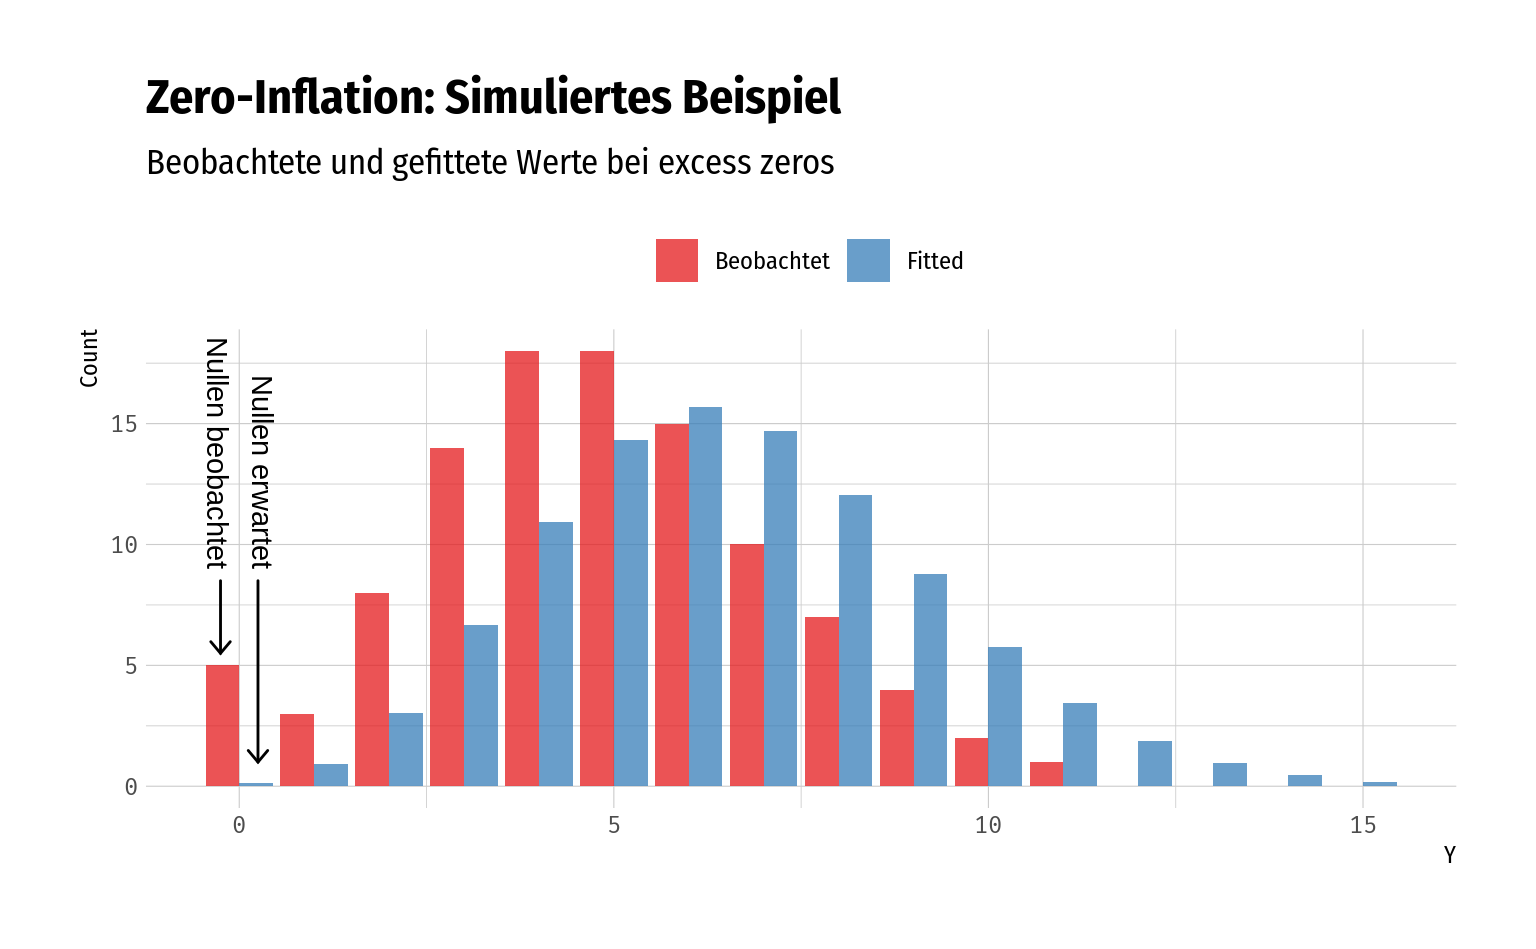
\includegraphics{poisson-regression_files/figure-latex/excess_zeros_viz-1} \end{center}

\hypertarget{vergleich-von-zero-inflated-models}{%
\subsubsection*{Vergleich von Zero-Inflated models}\label{vergleich-von-zero-inflated-models}}
\addcontentsline{toc}{subsubsection}{Vergleich von Zero-Inflated models}

Zum Vergleich zwischen Zählmodellen und ihren zero-inflated Gegenstücken (e.g.~Poisson vs.~ZIP oder NB vs.~ZINB) wird in der Literatur häufig der Vuong-Test \citep{vuongLikelihoodRatioTests1989, desmarais2013TestingZero} verwendet. Dieser Test ist explizit für den Vergleich von \textbf{un}geschachtelten Modellen entworfen (im Gegensatz zu z.B. dem Likelihood Ratio test). \citet{wilson2015MisuseVuong} kritisiert dieses Vorgehen mit der Begründung (und Demonstration), dass zero-inflated Modelle \emph{nicht} ungeschachtelt mit ihren ursprünglichen Zähmodellen sind. Auch \citet{perumean-chaneyZeroinflatedOverdispersedWhat2013} und \citet{hilbeModelingCountData2014}, die in diesem Dokument mehrfach zitiert werden, verwenden den Vuong-Test auf diese Weise.

Das Paper (\citet{wilson2015MisuseVuong}) ist recht kurz und definitiv einen Blick Wert, insbesondere da ich (Lukas) mir bisher nicht zutraue zu beurteilen, wer in dieser Frage \enquote{Recht} hat.

\begin{quote}
The misuse of the test stems from misunderstanding of what is meant by the terms \enquote{non-nested model} and \enquote{nested model}. As is the case with many frequently used terms their meanings are approximately understood by many, but precisely understood by few.

--- \citet{wilson2015MisuseVuong}, p.~52
\end{quote}

\hypertarget{modellierung}{%
\subsubsection*{Modellierung}\label{modellierung}}
\addcontentsline{toc}{subsubsection}{Modellierung}

Für die Modellierung von zero-inflated Daten stehen primär zwei Möglichkeiten zur Verfügung (vgl. auch \citet{hilbeModelingCountData2014}, p.~19):

\begin{enumerate}
\def\labelenumi{\arabic{enumi}.}
\tightlist
\item
  \emph{Zero-inflated models}: Mixture models, die aus zwei Wahrscheinlichkeitsfunktionen eine neue Wahrscheinlichkeitsfunktion generieren, die sowohl Nullen als auch positive counts beschreibt, allerdings nun auch einen \emph{zero-inflation}-Parameter hat (siehe Abschnitt \ref{mod-zi}).
\item
  \emph{Hurdle models}: Getrennte Modellierung von Nullen und positiven counts in zwei separaten Modellen (siehe Abschnitt \ref{mod-hurdle}).
\end{enumerate}

Ob hurdle model oder zero-inflated model die bessere Wahl ist hängt mitunter davon ab, welche Annahmen über die \emph{Ursache der Nullen} getroffen werden können.\\
Wenn es eine echte Trennung der Mechanismen (\emph{\enquote{separation of mechanisms}}) gibt, die die Nullen und die positiven counts verursachen, dann wäre ein hurdle model eher angemessen.\\
Wenn sich die Nullen überlappen, es also keine getrennten Prozesse zu geben scheint, dann wären zero-inflated models angemessen \citep[p.~209]{hilbeModelingCountData2014}.

Als Veranschaulichung für zwei sich überlappende Mechanismen können wir das \emph{fish}-Beispiel auf \href{https://stats.idre.ucla.edu/sas/output/zero-inflated-poisson-regression/}{dieser UCLA-Tutorialseite verwenden}. Hier ist die Anzahl der gefangenen Fische an einem Wochenende in einem Park die Zählvariable.

\begin{Shaded}
\begin{Highlighting}[]
\CommentTok{# Mittelwert & Varianz von 'count'}
\KeywordTok{describe_counts}\NormalTok{(fish}\OperatorTok{$}\NormalTok{count)}
\end{Highlighting}
\end{Shaded}

\begin{table}[H]
\centering
\begin{tabular}{rrrrl}
\toprule
N & Missing & Mittelwert & Varianz & Range\\
\midrule
250 & 0 & 3.3 & 135.37 & [0, 149]\\
\bottomrule
\end{tabular}
\end{table}

\begin{Shaded}
\begin{Highlighting}[]
\CommentTok{# Barchart für counts <= 50, Spannweite sehr groß}
\NormalTok{fish }\OperatorTok
\StringTok{  }\KeywordTok{filter}\NormalTok{(count }\OperatorTok{<=}\StringTok{ }\DecValTok{50}\NormalTok{) }\OperatorTok
\StringTok{  }\KeywordTok{ggplot}\NormalTok{(}\KeywordTok{aes}\NormalTok{(}\DataTypeTok{x =}\NormalTok{ count)) }\OperatorTok{+}
\StringTok{  }\KeywordTok{geom_bar}\NormalTok{(}\DataTypeTok{alpha =} \FloatTok{.75}\NormalTok{) }\OperatorTok{+}
\StringTok{  }\KeywordTok{scale_x_continuous}\NormalTok{() }\OperatorTok{+}
\StringTok{  }\KeywordTok{labs}\NormalTok{(}
    \DataTypeTok{title =} \StringTok{"'fish': Anzahl gefangener Fische"}\NormalTok{,}
    \DataTypeTok{subtitle =} \StringTok{"Limitiert auf counts unter 50"}\NormalTok{,}
    \DataTypeTok{x =} \StringTok{"Anzahl gefangener Fischer"}\NormalTok{, }\DataTypeTok{y =} \StringTok{"Count"}
\NormalTok{  )}
\end{Highlighting}
\end{Shaded}

\begin{center}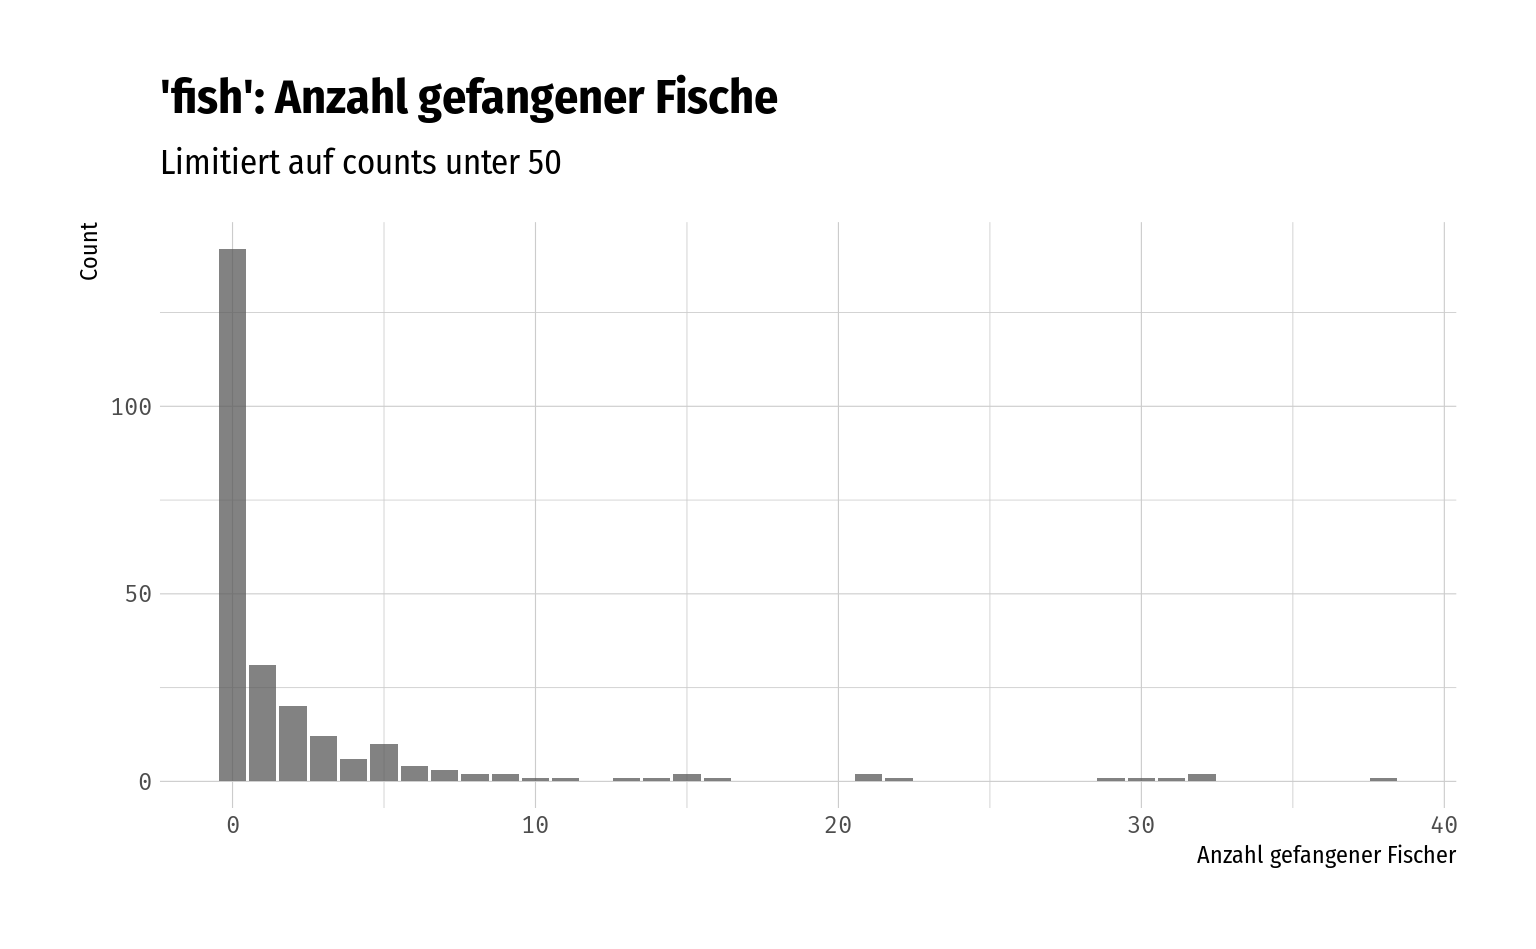
\includegraphics{poisson-regression_files/figure-latex/fishing_zeros-1} \end{center}

Die Anzahl der Nullen ist hier auffallend groß -- allerdings beobachten wir hier auch zwei unterschiedliche Mechanismen, die sich überlappen: Eine Gruppe kann das ganze Wochenende geangelt haben, während eine andere Gruppe gar nicht geangelt hat -- beide Gruppen werden jedoch am Ende nach der Anzahl ihrer gefangenen Fische befragt, weshalb wir in den Daten Nullen mit unterschiedlichem \enquote{Ursprung} erhalten

Da es hier nicht angemessen wäre, die Nullen und die positiven counts getrennt zu Modellieren, würden wir hier ein \emph{zero-inflated} Modell (z.B ZIP, ZINB, \ldots{}) verwenden.

\hypertarget{entscheidungshilfen}{%
\section{Entscheidungshilfen}\label{entscheidungshilfen}}

\citet{perumean-chaneyZeroinflatedOverdispersedWhat2013} schlagen folgendes Vorgehen vor um Overdispersion und Zero-Inflation zu erkennen:

\begin{center}\includegraphics{poisson-regression_files/figure-latex/perumean_chaney_decision_tree-1} \end{center}

Wobei im ersten Schritt sowohl Poisson als auch NB-Modelle gefittet werden, und dann nach Goodness-of-Fit (via LRT) (NB \textgreater{} Poisson?) entschieden wird.\\
Im zweiten Schritt werden die jeweiligen Modelle (entweder Poisson oder NB) mit ihren ZI-Counterparts verglichen (model fit, Vuong-Test), analog Schritt 1.\\
\enquote{LRT-Vuong Method}.

Eine allgemeinere Darstellung zur Veranschaulichung der sich ergebenden Möglichkeiten:

\begin{center}\includegraphics{poisson-regression_files/figure-latex/decision_tree-1} \end{center}

\hypertarget{appendix-appendix}{%
\appendix \addcontentsline{toc}{section}{\appendixname}}


\hypertarget{verfugbarkeit}{%
\section{Verfügbarkeit}\label{verfugbarkeit}}

Sowohl der Quelltext als auch das Output (sprich, dieses Dokument in mehreren Formaten) sind öffentlich an mehreren Orten zu finden:

\begin{table}[H]
\centering
\begin{tabular}{lll}
\toprule
  & Host & URL\\
\midrule
 & Gitea (self-hosted) & https://git.tadaa-data.de/lukas/poisson-regression\\
\cmidrule{2-3}
\multirow{-2}{*}{\raggedright\arraybackslash Code} & GitHub & https://github.com/jemus42/poisson-regression\\
\cmidrule{1-3}
 & GitHub Pages & https://jemus42.github.io/poisson-regression\\
\cmidrule{2-3}
\multirow{-2}{*}{\raggedright\arraybackslash Result} & Self-Hosted & https://lukas.tadaa-data.de/poisson/\\
\bottomrule
\end{tabular}
\end{table}

\hypertarget{erganzungen}{%
\section{Ergänzungen}\label{erganzungen}}

Hier finden sich Erläuterungen zu Themen, die nur tangentiell in Verbindung mit dem eigentlichen Thema stehen, aber unter Umständen dennoch von Interesse sein könnten.

\hypertarget{appendix-missingness}{%
\subsection{Missing values und missingness patterns}\label{appendix-missingness}}

Zu den Begriffen im Kontext von missingness wird folgende Unterscheidung bezüglich der Verteilung der missing values für eine Variable \(Y\) gemacht (vgl. auch \citet{littleStatisticalAnalysisMissing2002}, p.~12):

\begin{itemize}
\tightlist
\item
  \textbf{MCAR} (missing completely at random): Das Fehlen eines Wertes in \(Y\) ist völlig unabhängig von sowohl beobachteten als auch unbeobachtet Daten. Dieser Fall wäre der idealzustand, ist allerdings in der Regel weder realistisch noch verifizierbar.
\item
  \textbf{MAR} (missing at random): Es gibt einen Zusammenhang zwischen Ausfallwahrscheinlichkeit und \emph{beobachteten} Daten. Das heißt auch, dass missingness durch beobachtete Daten erklärt werden kann, weshalb dieser Fall noch akzeptabel wäre.
\item
  \textbf{MNAR} / \textbf{NMAR} (missing not at random): Weder \emph{MCAR} noch \emph{MAR} -- die Ausfallwahrscheinlichkeit hängt von \emph{unbeobachten} Daten ab. Das heißt, es gibt ein Ausfallmuster in \(Y\), das nicht durch vorliegende Daten erklärt werden kann, wodurch in der Regel verzerrte Effektschätzungen entstehen.
\end{itemize}

\hypertarget{trunc-cens}{%
\subsection{Truncation und Censoring}\label{trunc-cens}}

Wenn die Beobachtungen keine Nullen enthalten bzw. im Modell aus inhaltlichen Gründen nicht möglich sind, können \emph{zero-truncated} (ZT) Modelle verwendet werden. Diese Modelle sind insbesondere im Kontext von \emph{hurdle models} interessant (siehe Abschnitt \ref{mod-hurdle}), in denen die positiven counts getrennt von den Null-counts modelliert werden. Eine \emph{truncated} distribution wäre die zero-truncated Poisson (ZTP).

Bemerke, dass \emph{truncation} hier etwas anderes meint als \emph{censoring}:

\textbf{Truncation} bedeutet, dass bestimmte counts (i.e.~Merkmalsausprägungen in \(Y\)) \emph{nicht möglich} sind. Als Beispiel könnte die Dauer eines Krankenhausaufenthalts dienen, da Aufenthaltstage erst ab einem Tag aufgezeichnet werden. (siehe auch Datensatz \texttt{azprocedure}, \ref{data}).\\
Unterschieden werden kann zwischen \emph{left truncation} (z.B. keine counts kleiner als 5), \emph{right truncation} (analog, keine counts größer als 5), oder \emph{interval truncation} (nur counts im Intervall \([2, 10]\)).

\textbf{Censoring} wiederum bedeutet, dass eine Merkmalsausprägung (wie etwa \(Y = 0\) oder auch \(Y = 1029\)) zwar im Modell prinzipiell möglich ist, aber lediglich nicht in einer konkreten Stichprobe beobachtet wurde.

\hypertarget{mod-hurdle}{%
\subsection{Hurdle models}\label{mod-hurdle}}

Die nachfolgende Beschreibung dient daher eher der Vollständigkeit, da hurdle models in bestimmten Anwendungsgebieten scheinbar recht populär sind -- allerdings ist es vermutlich eher schwierig sie auf binäre outcomes anzuwenden.

Im Allgemeinen kann man zwei Arten von hurdle models unterscheiden, die jeweils aus zwei Modellkomponenten bestehen:

\begin{itemize}
\tightlist
\item
  \emph{Nested} hurdle models: Beide Komponenten nested (e.g.~beide Poisson).
\item
  \emph{Non-nested} hurdle models: Hurdle-Komponente als vollständig anderer Prozess betrachtet und via e.g.~logit modelliert.
\end{itemize}

Zwei gängige Komponenten für unnested hurdle models:

\begin{enumerate}
\def\labelenumi{\arabic{enumi}.}
\tightlist
\item
  Binary 0,1 response, (logit oder probit)

  \begin{itemize}
  \tightlist
  \item
    Modellierung der Wahrscheinlichkeit für die non-zero counts
  \end{itemize}
\item
  Zero-truncated count model
\end{enumerate}

\begin{itemize}
\tightlist
\item
  Erlauben sowohl under- als auch overdispersion
\item
  (Unnested models) erlauben systematischen Unterschied im Prozess, der zu e.g.~Outcomes = 0 vs.~Outcomes \textgreater{} 0 führt, was durch die Wahl unterschiedlicher Modelle für beide Komponenten abgebildet wird
\end{itemize}

In diesem Fall entspricht das Resultat eines hurdle models zwei separat gefitteten Modellen (e.g.~Pois + Logit), die getrennt interpretierbar sind (im Gegensatz zu zero-inflated models!).

\BeginKnitrBlock{definition}[Hurdle Model]
\protect\hypertarget{def:unnamed-chunk-5}{}{\label{def:unnamed-chunk-5} \iffalse (Hurdle Model) \fi{} }Nach \citet{winkelmannEconometricAnalysisCount2010}, p.~179f:

Sei \(g_1(0)\) die Wahrscheinlichkeit des Outcomes \(0\) und \(g_1(k), k = 1, 2, 3, \ldots\) die Wahrscheinlichkeitsfunktion für natürliche Zahlen, dann ist die Wahrscheinlichkeitsfunktion eines \emph{hurdle-at-zero} Modells:

\begin{align*}
f(y = 0) &= g_1(0) \\
f(y = k) &= (1 - g_1(0)) g_2(k), \quad k = 1, 2, 3, \ldots
\end{align*}

Bzw. nach \citet{mullahy1986SpecificationTesting} mit \(f_1\) und \(f_2\) als PMFs für natürliche Zahlen

\begin{align*}
f(y = 0) &= f_1(0) \\
f(y = 1) &= \frac{1 - f_1(0)}{1 - f_2(0)} f_2(k) \\
         &= \Theta f_2(k), \quad k = 1, 2, 3, \ldots 
\end{align*}

Wobei

\begin{itemize}
\tightlist
\item
  \(f_2\) als \emph{parent process} bezeichnet wird
\item
  \(1 - f_1(0)\) die Wahrscheinlichkeit angibt, die Hürde (\(y = 0\)) zu \enquote{überqueren} (\emph{\enquote{crossing the hurdle}}).
\item
  \(1 - f_2(0)\) zur Normalisierung von \(f_2\) dient, um deren truncation zu berücksichtigen.
\end{itemize}

Der Erwartungswert des hurdle models ist

\[
  \mathbb{E}_h(y) = \Theta \sum_{k=1}^\infty k f_2(k) = \Theta \mathbb{E}_2(y)
\]

Mit \(\mathbb{E}_2\) als Erwartunsgwert von \(f_2\).

Mit \(f_2 = \mathrm{Poisson}\):

\begin{itemize}
\tightlist
\item
  \(0 < \Theta < 1\): Overdispersion\\
\item
  \(1 < \Theta < \frac{\lambda_2 + 1}{\lambda_2}\): Underdispersion
\end{itemize}
\EndKnitrBlock{definition}

\begin{quote}
\enquote{By far the most popular hurdle model in practice is the hurdle-at-zero negative bonomial model}
\citep[p.~183]{winkelmannEconometricAnalysisCount2010}
\end{quote}

mit \(f_1 \sim NB(\beta_1, \alpha_1)\) und \(f_2 \sim NB(\beta_2, \alpha_2)\)

\hypertarget{repro}{%
\section{Reproduzierbarkeit}\label{repro}}

\hypertarget{r-code}{%
\subsection{R-Code}\label{r-code}}

Hier verwendeter Code profitiert stark vom \href{https://www.tidyverse.org/}{\texttt{tidyverse}}.\\
Insbesondere wird anstelle der Funktion \texttt{data.frame} in der Regel \texttt{tibble} (package \texttt{tibble}, automatisch re-exportiert von \texttt{dplyr}) verwendet. Diese Alternative bietet einige quality of life improvements für schnelle Simulationen, zum Beispiel die Verwendung von Variablen während diese noch definiert werden:

\begin{Shaded}
\begin{Highlighting}[]
\CommentTok{# Nicht möglich:}
\KeywordTok{data.frame}\NormalTok{(}
   \DataTypeTok{x1 =} \KeywordTok{rnorm}\NormalTok{(}\DecValTok{10}\NormalTok{),}
   \DataTypeTok{x2 =} \KeywordTok{rnorm}\NormalTok{(}\DecValTok{10}\NormalTok{, }\DataTypeTok{mean =} \DecValTok{5}\NormalTok{),}
   \DataTypeTok{y =} \DecValTok{50} \OperatorTok{+}\StringTok{ }\DecValTok{3} \OperatorTok{*}\StringTok{ }\NormalTok{x1 }\OperatorTok{+}\StringTok{ }\DecValTok{5} \OperatorTok{*}\StringTok{ }\NormalTok{x2}
\NormalTok{)}

\CommentTok{# Funktioniert!}
\KeywordTok{tibble}\NormalTok{(}
   \DataTypeTok{x1 =} \KeywordTok{rnorm}\NormalTok{(}\DecValTok{10}\NormalTok{),}
   \DataTypeTok{x2 =} \KeywordTok{rnorm}\NormalTok{(}\DecValTok{10}\NormalTok{, }\DataTypeTok{mean =} \DecValTok{5}\NormalTok{),}
   \DataTypeTok{y =} \DecValTok{50} \OperatorTok{+}\StringTok{ }\DecValTok{3} \OperatorTok{*}\StringTok{ }\NormalTok{x1 }\OperatorTok{+}\StringTok{ }\DecValTok{5} \OperatorTok{*}\StringTok{ }\NormalTok{x2}
\NormalTok{)}
\end{Highlighting}
\end{Shaded}

Zusätzlich kann die Pipe (\texttt{\%\textgreater{}\%}) Verwendung finden, ein function composition operator.\\
Es gilt:

\texttt{f(g(h(x),\ b\ =\ 4),\ a\ =\ 1)} = \texttt{h(x)\ \%\textgreater{}\%\ g(b\ =\ 4)\ \%\textgreater{}\%\ f(a\ =\ 1)}

\begin{Shaded}
\begin{Highlighting}[]
\CommentTok{# Klassisch}
\NormalTok{x <-}\StringTok{ }\KeywordTok{rnorm}\NormalTok{(}\DecValTok{100}\NormalTok{, }\DataTypeTok{mean =} \DecValTok{15}\NormalTok{)}
\NormalTok{x_mean <-}\StringTok{ }\KeywordTok{mean}\NormalTok{(x)}
\KeywordTok{sqrt}\NormalTok{(x_mean)}

\CommentTok{# oder}
\KeywordTok{sqrt}\NormalTok{(}\KeywordTok{mean}\NormalTok{(}\KeywordTok{rnorm}\NormalTok{(}\DecValTok{100}\NormalTok{, }\DataTypeTok{mean =} \DecValTok{15}\NormalTok{)))}

\CommentTok{# piped}
\KeywordTok{rnorm}\NormalTok{(}\DecValTok{100}\NormalTok{, }\DataTypeTok{mean =} \DecValTok{15}\NormalTok{) }\OperatorTok
\StringTok{   }\KeywordTok{mean}\NormalTok{() }\OperatorTok
\StringTok{   }\KeywordTok{sqrt}\NormalTok{()}

\CommentTok{# Klassisch}
\NormalTok{iris_subset <-}\StringTok{ }\KeywordTok{subset}\NormalTok{(iris, Species }\OperatorTok{==}\StringTok{ "setosa"}\NormalTok{)}
\KeywordTok{head}\NormalTok{(iris_subset[}\KeywordTok{order}\NormalTok{(iris_subset}\OperatorTok{$}\NormalTok{Sepal.Length, }\DataTypeTok{decreasing =} \OtherTok{TRUE}\NormalTok{), ], }\DataTypeTok{n =} \DecValTok{5}\NormalTok{)}

\CommentTok{# tidyverse-style (incl. filter() als subset()-Analog und top_n() für order() + head())}
\NormalTok{iris }\OperatorTok
\StringTok{   }\KeywordTok{filter}\NormalTok{(Species }\OperatorTok{==}\StringTok{ "setosa"}\NormalTok{) }\OperatorTok
\StringTok{   }\KeywordTok{top_n}\NormalTok{(Sepal.Length, }\DataTypeTok{n =} \DecValTok{5}\NormalTok{)}
\end{Highlighting}
\end{Shaded}

Letztlich stellt das Package \href{https://broom.tidyverse.org/}{\texttt{broom}} eine wichtige Ergänzung dar. Mitunter ist \href{https://broom.tidyverse.org/reference/augment.lm.html\#examples}{\texttt{augment()}} eine komfortable Möglichkeit um schnell in tabellarischer Form gefittete Werte mit ihren dazugehörigen x-Werten zu erhalten.

\hypertarget{session-info}{%
\subsection{Session Info}\label{session-info}}

\begin{table}[H]
\centering
\begin{tabular}{ll}
\toprule
Umgebungsvariable & Wert\\
\midrule
version & R version 3.6.1 (2017-01-27)\\
os & Ubuntu 16.04.6 LTS\\
system & x86\_64, linux-gnu\\
ui & X11\\
language & en\_US.UTF-8\\
collate & en\_US.UTF-8\\
ctype & en\_US.UTF-8\\
tz & UTC\\
date & 2019-09-11\\
\bottomrule
\end{tabular}
\end{table}

\begin{table}[H]
\centering
\begin{tabular}{lll}
\toprule
Package & Version & Quelle\\
\midrule
broom & 0.5.2 & CRAN (R 3.6.1)\\
DiagrammeR & 1.0.1 & CRAN (R 3.6.1)\\
dplyr & 0.8.3 & CRAN (R 3.6.1)\\
firasans & 0.1.0 & Github (hrbrmstr/firasans@52f83c8)\\
gamlss & 5.1-4 & CRAN (R 3.6.1)\\
gamlss.data & 5.1-4 & CRAN (R 3.6.1)\\
gamlss.dist & 5.1-4 & CRAN (R 3.6.1)\\
ggplot2 & 3.2.1 & CRAN (R 3.6.1)\\
hrbrthemes & 0.6.0 & CRAN (R 3.6.1)\\
kableExtra & 1.1.0 & CRAN (R 3.6.1)\\
MASS & 7.3-51.4 & CRAN (R 3.6.1)\\
nlme & 3.1-140 & CRAN (R 3.6.1)\\
pander & 0.6.3 & CRAN (R 3.6.1)\\
purrr & 0.3.2 & CRAN (R 3.6.1)\\
tidyr & 0.8.3 & CRAN (R 3.6.1)\\
VGAM & 1.1-1 & CRAN (R 3.6.1)\\
\bottomrule
\end{tabular}
\end{table}

\hypertarget{unsorted}{%
\subsection{Unsorted}\label{unsorted}}

Hier liegen temporär Opfer der Umstrukturierung, bis sie ein passendes zu Hause gefunden haben, oder auf die farm upstate umziehen.

\hypertarget{general-advice}{%
\subsubsection{General Advice}\label{general-advice}}

\begin{itemize}
\tightlist
\item
  Starte mit einem Poisson-Modell und baue darauf auf
\item
  Benutze robuste Varianzschätzer (e.g.~sandwich, Bootstrap-SEs sind meist den Aufwand nicht wert) -- entweder sie helfen, oder sie schaden nicht.
\item
  Das gängigste Problem ist overdispersion, aber nicht jede overdispersion ist gleich.
\item
  Die erwartete Anzahl an Nullen (unter Poisson) ist \(\exp(-\bar{x}) \cdot n\)
\end{itemize}

\hypertarget{beispiel-nach-hilbemodelingcountdata2014-p.211ff}{%
\subsubsection{\texorpdfstring{Beispiel nach \citet{hilbeModelingCountData2014}, p.~211ff}{Beispiel nach @hilbeModelingCountData2014, p.~211ff}}\label{beispiel-nach-hilbemodelingcountdata2014-p.211ff}}

(Eigentlich kompliziertes Beispiel, weil 0 counts nicht möglich sind, müsste man truncated drangehen)

Grundlage ist der Datensatz \texttt{azprocedure} (siehe Abschnitt \ref{data}) zur Dauer des Krankenhausaufenthalts.

Zuerst werfen wir einen Blick auf die Daten und fitten ein reguläres Poissonmodell.

\begin{Shaded}
\begin{Highlighting}[]
\KeywordTok{data}\NormalTok{(azprocedure, }\DataTypeTok{package =} \StringTok{"COUNT"}\NormalTok{)}

\KeywordTok{describe_counts}\NormalTok{(azprocedure}\OperatorTok{$}\NormalTok{los)}
\end{Highlighting}
\end{Shaded}

\begin{table}[H]
\centering
\begin{tabular}{rrrrl}
\toprule
N & Missing & Mittelwert & Varianz & Range\\
\midrule
3589 & 0 & 8.83 & 47.97 & [1, 83]\\
\bottomrule
\end{tabular}
\end{table}

\begin{Shaded}
\begin{Highlighting}[]
\CommentTok{# Barchart: So grob poissonverteilt?}
\KeywordTok{ggplot}\NormalTok{(}\DataTypeTok{data =}\NormalTok{ azprocedure, }\KeywordTok{aes}\NormalTok{(}\DataTypeTok{x =}\NormalTok{ los)) }\OperatorTok{+}
\StringTok{  }\KeywordTok{geom_bar}\NormalTok{(}\DataTypeTok{alpha =} \FloatTok{.75}\NormalTok{) }\OperatorTok{+}
\StringTok{  }\KeywordTok{labs}\NormalTok{(}
    \DataTypeTok{title =} \StringTok{"Hospital length of stay (LOS)"}\NormalTok{,}
    \DataTypeTok{subtitle =} \StringTok{"azprocedure data (Hilbe 2014)"}\NormalTok{,}
    \DataTypeTok{x =} \StringTok{"LOS"}\NormalTok{, }\DataTypeTok{y =} \StringTok{"Count"} 
\NormalTok{  )}
\end{Highlighting}
\end{Shaded}

\begin{center}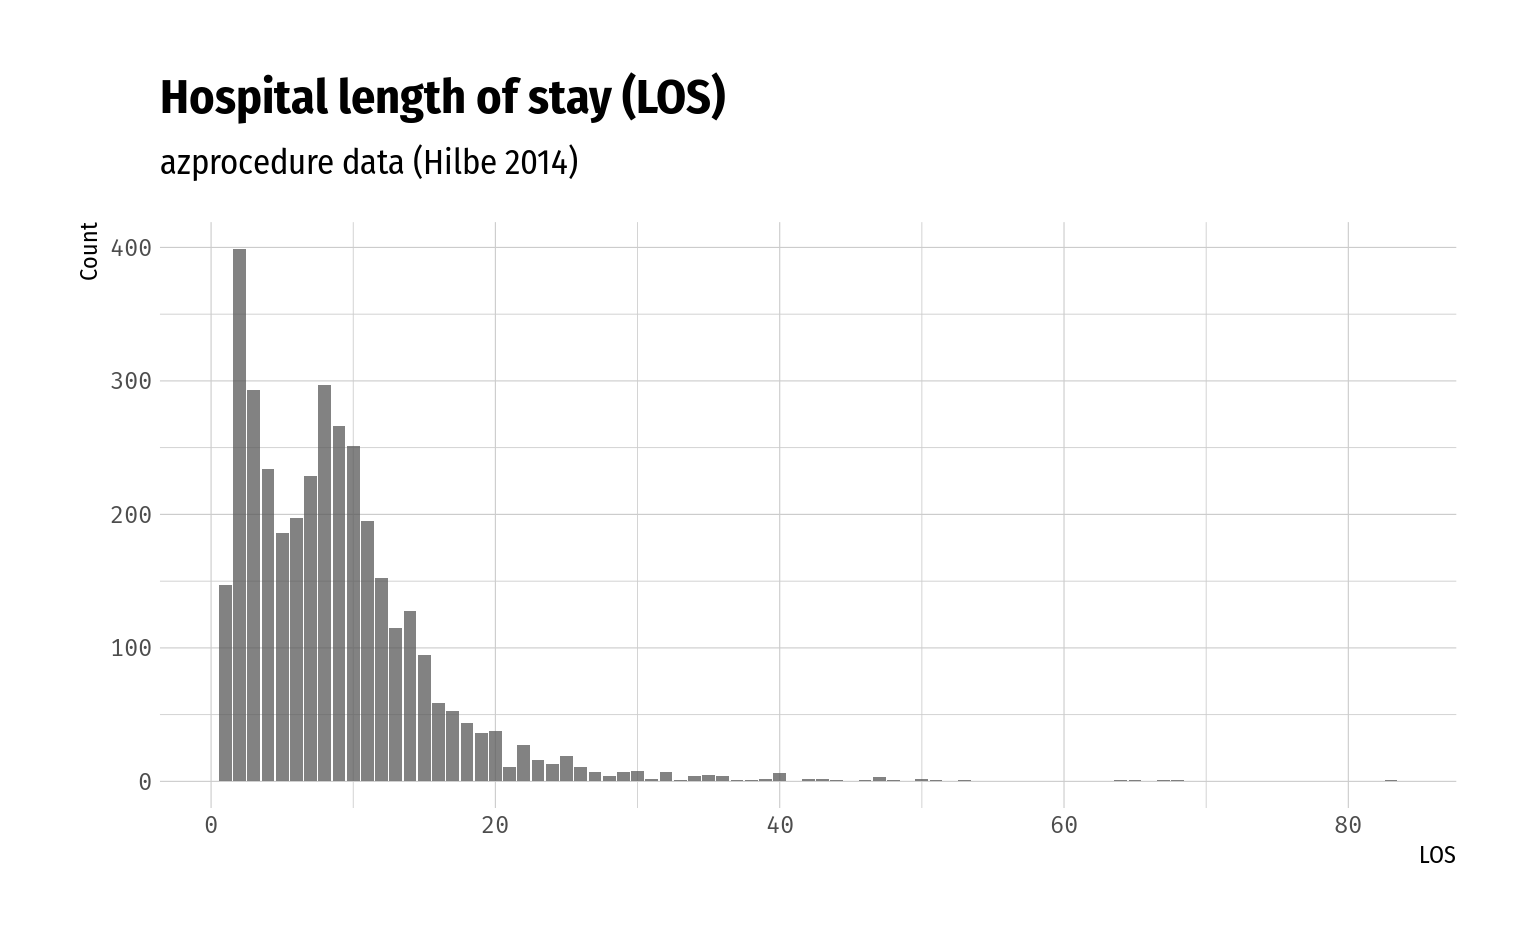
\includegraphics{poisson-regression_files/figure-latex/underdisp-azprocedure-over-1} \end{center}

\begin{Shaded}
\begin{Highlighting}[]
\CommentTok{# Model fit}
\NormalTok{model_azproc <-}\StringTok{ }\KeywordTok{glm}\NormalTok{(los }\OperatorTok{~}\StringTok{ }\NormalTok{procedure }\OperatorTok{+}\StringTok{ }\NormalTok{sex }\OperatorTok{+}\StringTok{ }\NormalTok{admit, }
                    \DataTypeTok{data =}\NormalTok{ azprocedure, }\DataTypeTok{family =} \KeywordTok{poisson}\NormalTok{())}
 
\CommentTok{# Model output (ohne exponentierte Koeffizienten)}
\KeywordTok{pander}\NormalTok{(model_azproc)}
\end{Highlighting}
\end{Shaded}

\begin{longtable}[]{@{}ccccc@{}}
\caption{Fitting generalized (poisson/log) linear model: los \textasciitilde{} procedure + sex + admit}\tabularnewline
\toprule
\begin{minipage}[b]{0.21\columnwidth}\centering
~\strut
\end{minipage} & \begin{minipage}[b]{0.13\columnwidth}\centering
Estimate\strut
\end{minipage} & \begin{minipage}[b]{0.16\columnwidth}\centering
Std. Error\strut
\end{minipage} & \begin{minipage}[b]{0.12\columnwidth}\centering
z value\strut
\end{minipage} & \begin{minipage}[b]{0.14\columnwidth}\centering
Pr(\textgreater{}\textbar{}z\textbar{})\strut
\end{minipage}\tabularnewline
\midrule
\endfirsthead
\toprule
\begin{minipage}[b]{0.21\columnwidth}\centering
~\strut
\end{minipage} & \begin{minipage}[b]{0.13\columnwidth}\centering
Estimate\strut
\end{minipage} & \begin{minipage}[b]{0.16\columnwidth}\centering
Std. Error\strut
\end{minipage} & \begin{minipage}[b]{0.12\columnwidth}\centering
z value\strut
\end{minipage} & \begin{minipage}[b]{0.14\columnwidth}\centering
Pr(\textgreater{}\textbar{}z\textbar{})\strut
\end{minipage}\tabularnewline
\midrule
\endhead
\begin{minipage}[t]{0.21\columnwidth}\centering
\textbf{(Intercept)}\strut
\end{minipage} & \begin{minipage}[t]{0.13\columnwidth}\centering
1.491\strut
\end{minipage} & \begin{minipage}[t]{0.16\columnwidth}\centering
0.01539\strut
\end{minipage} & \begin{minipage}[t]{0.12\columnwidth}\centering
96.91\strut
\end{minipage} & \begin{minipage}[t]{0.14\columnwidth}\centering
0\strut
\end{minipage}\tabularnewline
\begin{minipage}[t]{0.21\columnwidth}\centering
\textbf{procedure}\strut
\end{minipage} & \begin{minipage}[t]{0.13\columnwidth}\centering
0.9574\strut
\end{minipage} & \begin{minipage}[t]{0.16\columnwidth}\centering
0.01218\strut
\end{minipage} & \begin{minipage}[t]{0.12\columnwidth}\centering
78.61\strut
\end{minipage} & \begin{minipage}[t]{0.14\columnwidth}\centering
0\strut
\end{minipage}\tabularnewline
\begin{minipage}[t]{0.21\columnwidth}\centering
\textbf{sex}\strut
\end{minipage} & \begin{minipage}[t]{0.13\columnwidth}\centering
-0.1302\strut
\end{minipage} & \begin{minipage}[t]{0.16\columnwidth}\centering
0.01179\strut
\end{minipage} & \begin{minipage}[t]{0.12\columnwidth}\centering
-11.04\strut
\end{minipage} & \begin{minipage}[t]{0.14\columnwidth}\centering
2.408e-28\strut
\end{minipage}\tabularnewline
\begin{minipage}[t]{0.21\columnwidth}\centering
\textbf{admit}\strut
\end{minipage} & \begin{minipage}[t]{0.13\columnwidth}\centering
0.3331\strut
\end{minipage} & \begin{minipage}[t]{0.16\columnwidth}\centering
0.0121\strut
\end{minipage} & \begin{minipage}[t]{0.12\columnwidth}\centering
27.52\strut
\end{minipage} & \begin{minipage}[t]{0.14\columnwidth}\centering
1.11e-166\strut
\end{minipage}\tabularnewline
\bottomrule
\end{longtable}

\begin{Shaded}
\begin{Highlighting}[]
\CommentTok{# Pearson Dispersion:}
\KeywordTok{dispersion}\NormalTok{(model_azproc)}
\end{Highlighting}
\end{Shaded}

\begin{verbatim}
#> X-squared(3585) = 11588.08
#> Pearson Dispersion = 3.232
\end{verbatim}

Der Dispersionsindex lässt auf overdispersion schließen.\\
Betrachten wir ein Subset der Daten, indem wir nur Beobachtungen mit \(\mathtt{LOS} \le 8\) betrachten, erhalten wir ein anderes Bild:

\begin{Shaded}
\begin{Highlighting}[]
\NormalTok{azprocedure_subset <-}\StringTok{ }\KeywordTok{subset}\NormalTok{(azprocedure, los }\OperatorTok{<=}\StringTok{ }\DecValTok{8}\NormalTok{)}

\KeywordTok{describe_counts}\NormalTok{(azprocedure_subset}\OperatorTok{$}\NormalTok{los)}
\end{Highlighting}
\end{Shaded}

\begin{table}[H]
\centering
\begin{tabular}{rrrrl}
\toprule
N & Missing & Mittelwert & Varianz & Range\\
\midrule
1982 & 0 & 4.47 & 5.34 & [1, 8]\\
\bottomrule
\end{tabular}
\end{table}

\begin{Shaded}
\begin{Highlighting}[]
\CommentTok{# Barchart}
\KeywordTok{ggplot}\NormalTok{(}\DataTypeTok{data =}\NormalTok{ azprocedure_subset, }\KeywordTok{aes}\NormalTok{(}\DataTypeTok{x =}\NormalTok{ los)) }\OperatorTok{+}
\StringTok{  }\KeywordTok{geom_bar}\NormalTok{(}\DataTypeTok{alpha =} \FloatTok{.75}\NormalTok{) }\OperatorTok{+}
\StringTok{  }\KeywordTok{labs}\NormalTok{(}
    \DataTypeTok{title =} \StringTok{"Hospital length of stay (LOS)"}\NormalTok{,}
    \DataTypeTok{subtitle =} \StringTok{"Subset (LOS <= 8) der azprocedure data (Hilbe 2014)"}\NormalTok{,}
    \DataTypeTok{x =} \StringTok{"LOS"}\NormalTok{, }\DataTypeTok{y =} \StringTok{"Count"} 
\NormalTok{  )}
\end{Highlighting}
\end{Shaded}

\begin{center}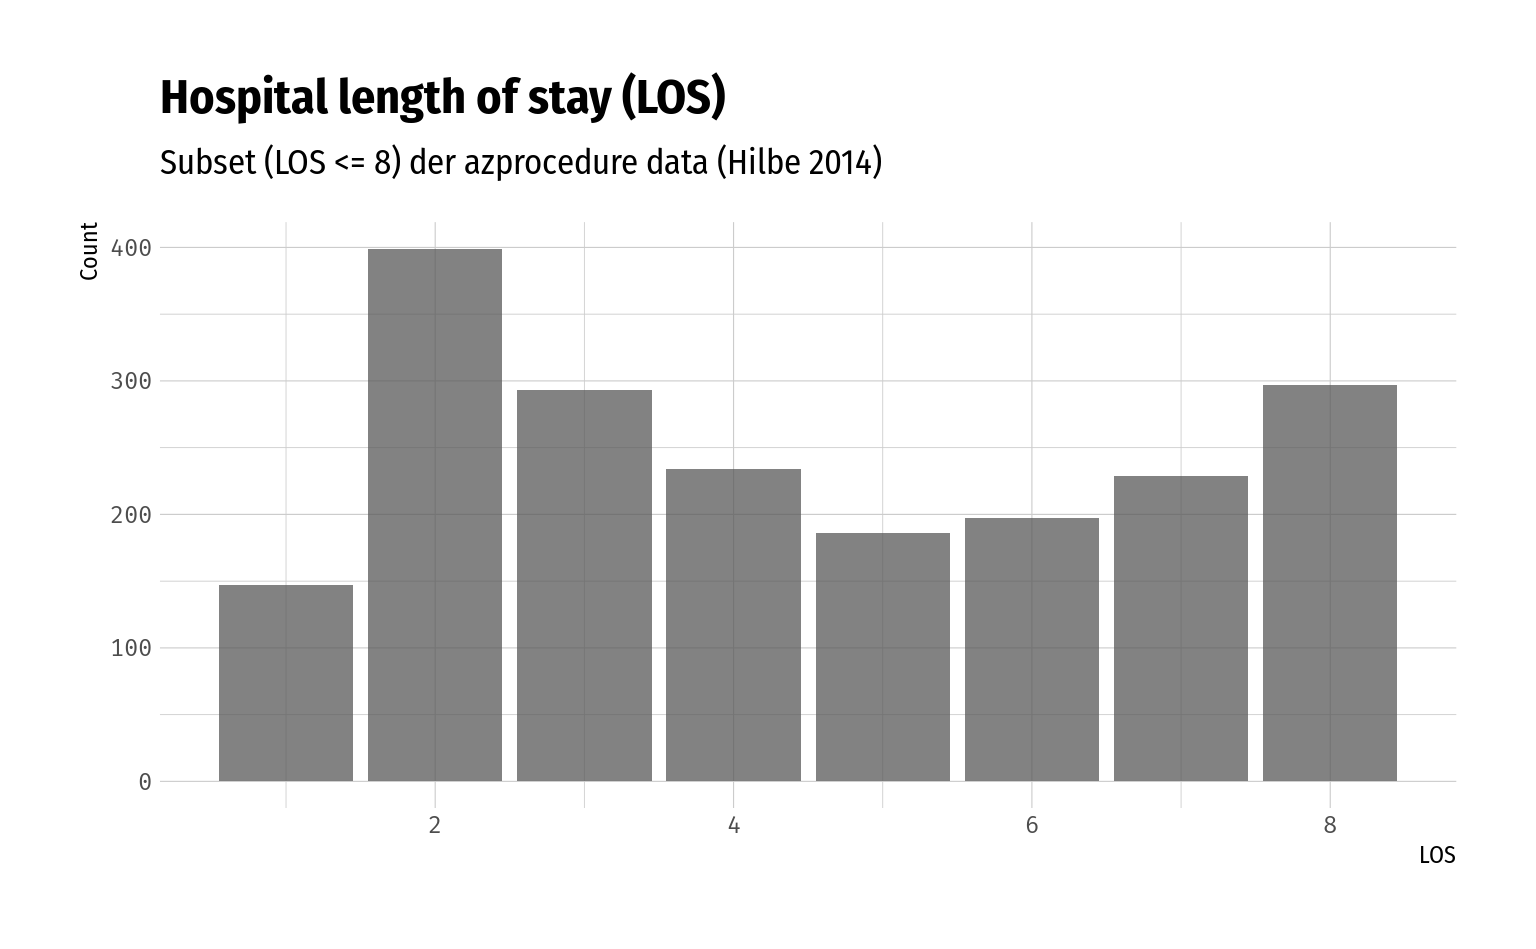
\includegraphics{poisson-regression_files/figure-latex/underdisp-azprocedure_under-1} \end{center}

\begin{Shaded}
\begin{Highlighting}[]
\NormalTok{model_azproc_u <-}\StringTok{ }\KeywordTok{glm}\NormalTok{(los }\OperatorTok{~}\StringTok{ }\NormalTok{procedure }\OperatorTok{+}\StringTok{ }\NormalTok{sex }\OperatorTok{+}\StringTok{ }\NormalTok{admit, }
                      \DataTypeTok{data =}\NormalTok{ azprocedure_subset, }\DataTypeTok{family =} \KeywordTok{poisson}\NormalTok{())}

\KeywordTok{pander}\NormalTok{(model_azproc_u)}
\end{Highlighting}
\end{Shaded}

\begin{longtable}[]{@{}ccccc@{}}
\caption{Fitting generalized (poisson/log) linear model: los \textasciitilde{} procedure + sex + admit}\tabularnewline
\toprule
\begin{minipage}[b]{0.21\columnwidth}\centering
~\strut
\end{minipage} & \begin{minipage}[b]{0.13\columnwidth}\centering
Estimate\strut
\end{minipage} & \begin{minipage}[b]{0.16\columnwidth}\centering
Std. Error\strut
\end{minipage} & \begin{minipage}[b]{0.12\columnwidth}\centering
z value\strut
\end{minipage} & \begin{minipage}[b]{0.16\columnwidth}\centering
Pr(\textgreater{}\textbar{}z\textbar{})\strut
\end{minipage}\tabularnewline
\midrule
\endfirsthead
\toprule
\begin{minipage}[b]{0.21\columnwidth}\centering
~\strut
\end{minipage} & \begin{minipage}[b]{0.13\columnwidth}\centering
Estimate\strut
\end{minipage} & \begin{minipage}[b]{0.16\columnwidth}\centering
Std. Error\strut
\end{minipage} & \begin{minipage}[b]{0.12\columnwidth}\centering
z value\strut
\end{minipage} & \begin{minipage}[b]{0.16\columnwidth}\centering
Pr(\textgreater{}\textbar{}z\textbar{})\strut
\end{minipage}\tabularnewline
\midrule
\endhead
\begin{minipage}[t]{0.21\columnwidth}\centering
\textbf{(Intercept)}\strut
\end{minipage} & \begin{minipage}[t]{0.13\columnwidth}\centering
1.187\strut
\end{minipage} & \begin{minipage}[t]{0.16\columnwidth}\centering
0.02498\strut
\end{minipage} & \begin{minipage}[t]{0.12\columnwidth}\centering
47.52\strut
\end{minipage} & \begin{minipage}[t]{0.16\columnwidth}\centering
0\strut
\end{minipage}\tabularnewline
\begin{minipage}[t]{0.21\columnwidth}\centering
\textbf{procedure}\strut
\end{minipage} & \begin{minipage}[t]{0.13\columnwidth}\centering
0.731\strut
\end{minipage} & \begin{minipage}[t]{0.16\columnwidth}\centering
0.02398\strut
\end{minipage} & \begin{minipage}[t]{0.12\columnwidth}\centering
30.48\strut
\end{minipage} & \begin{minipage}[t]{0.16\columnwidth}\centering
4.848e-204\strut
\end{minipage}\tabularnewline
\begin{minipage}[t]{0.21\columnwidth}\centering
\textbf{sex}\strut
\end{minipage} & \begin{minipage}[t]{0.13\columnwidth}\centering
-0.06892\strut
\end{minipage} & \begin{minipage}[t]{0.16\columnwidth}\centering
0.02294\strut
\end{minipage} & \begin{minipage}[t]{0.12\columnwidth}\centering
-3.004\strut
\end{minipage} & \begin{minipage}[t]{0.16\columnwidth}\centering
0.00266\strut
\end{minipage}\tabularnewline
\begin{minipage}[t]{0.21\columnwidth}\centering
\textbf{admit}\strut
\end{minipage} & \begin{minipage}[t]{0.13\columnwidth}\centering
0.3097\strut
\end{minipage} & \begin{minipage}[t]{0.16\columnwidth}\centering
0.02236\strut
\end{minipage} & \begin{minipage}[t]{0.12\columnwidth}\centering
13.85\strut
\end{minipage} & \begin{minipage}[t]{0.16\columnwidth}\centering
1.286e-43\strut
\end{minipage}\tabularnewline
\bottomrule
\end{longtable}

\begin{Shaded}
\begin{Highlighting}[]
\KeywordTok{dispersion}\NormalTok{(model_azproc_u)}
\end{Highlighting}
\end{Shaded}

\begin{verbatim}
#> X-squared(1978) = 1562.75
#> Pearson Dispersion = 0.790
\end{verbatim}

In diesem Fall haben wir es mit underdispersion zu tun, also versuchen wir es mal mit der GP:

\begin{Shaded}
\begin{Highlighting}[]
\KeywordTok{library}\NormalTok{(VGAM)}
\KeywordTok{library}\NormalTok{(gamlss)}

\NormalTok{mod_gp_vgam <-}\StringTok{ }\KeywordTok{vglm}\NormalTok{(los }\OperatorTok{~}\StringTok{ }\NormalTok{procedure }\OperatorTok{+}\StringTok{ }\NormalTok{sex }\OperatorTok{+}\StringTok{ }\NormalTok{admit, }\DataTypeTok{data =}\NormalTok{ azprocedure_subset, }\DataTypeTok{family =} \KeywordTok{genpoisson}\NormalTok{())}

\NormalTok{mod_gp_gamlss <-}\StringTok{ }\KeywordTok{gamlss}\NormalTok{(los }\OperatorTok{~}\StringTok{ }\NormalTok{procedure }\OperatorTok{+}\StringTok{ }\NormalTok{sex }\OperatorTok{+}\StringTok{ }\NormalTok{admit, }\DataTypeTok{data =}\NormalTok{ azprocedure_subset, }\DataTypeTok{family =} \KeywordTok{GPO}\NormalTok{())}
\end{Highlighting}
\end{Shaded}

\begin{verbatim}
#> GAMLSS-RS iteration 1: Global Deviance = 7969.342 
#> GAMLSS-RS iteration 2: Global Deviance = 7961.567 
#> GAMLSS-RS iteration 3: Global Deviance = 7961.567
\end{verbatim}

\begin{Shaded}
\begin{Highlighting}[]
\KeywordTok{summary}\NormalTok{(mod_gp_vgam)}
\end{Highlighting}
\end{Shaded}

\begin{verbatim}
#> 
#> Call:
#> vglm(formula = los ~ procedure + sex + admit, family = genpoisson(), 
#>     data = azprocedure_subset)
#> 
#> Pearson residuals:
#>                        Min      1Q   Median     3Q   Max
#> rhobitlink(lambda) -0.6573 -0.5912 -0.28788 0.2773 6.782
#> loglink(theta)     -2.3158 -0.6304  0.07304 0.8734 1.627
#> 
#> Coefficients: 
#>               Estimate Std. Error z value Pr(>|z|)    
#> (Intercept):1 -0.24021    0.03523  -6.819 9.16e-12 ***
#> (Intercept):2  1.30125    0.02766  47.042  < 2e-16 ***
#> procedure      0.71846    0.02143  33.521  < 2e-16 ***
#> sex           -0.06760    0.02043  -3.308 0.000939 ***
#> admit          0.31193    0.01993  15.652  < 2e-16 ***
#> ---
#> Signif. codes:  0 '***' 0.001 '**' 0.01 '*' 0.05 '.' 0.1 ' ' 1
#> 
#> Names of linear predictors: rhobitlink(lambda), loglink(theta)
#> 
#> Log-likelihood: -3956.379 on 3959 degrees of freedom
#> 
#> Number of Fisher scoring iterations: 6 
#> 
#> No Hauck-Donner effect found in any of the estimates
\end{verbatim}

\begin{Shaded}
\begin{Highlighting}[]
\KeywordTok{summary}\NormalTok{(mod_gp_gamlss)}
\end{Highlighting}
\end{Shaded}

\begin{verbatim}
#> ******************************************************************
#> Family:  c("GPO", "Generalised Poisson") 
#> 
#> Call:  gamlss(formula = los ~ procedure + sex + admit, family = GPO(),  
#>     data = azprocedure_subset) 
#> 
#> Fitting method: RS() 
#> 
#> ------------------------------------------------------------------
#> Mu link function:  log
#> Mu Coefficients:
#>             Estimate Std. Error t value Pr(>|t|)    
#> (Intercept)  1.18687    0.02980  39.824   <2e-16 ***
#> procedure    0.73075    0.03959  18.456   <2e-16 ***
#> sex         -0.06892    0.02643  -2.607   0.0092 ** 
#> admit        0.30974    0.02750  11.264   <2e-16 ***
#> ---
#> Signif. codes:  0 '***' 0.001 '**' 0.01 '*' 0.05 '.' 0.1 ' ' 1
#> 
#> ------------------------------------------------------------------
#> Sigma link function:  log
#> Sigma Coefficients:
#>             Estimate Std. Error t value Pr(>|t|)
#> (Intercept)   -36.04    2246.20  -0.016    0.987
#> 
#> ------------------------------------------------------------------
#> No. of observations in the fit:  1982 
#> Degrees of Freedom for the fit:  5
#>       Residual Deg. of Freedom:  1977 
#>                       at cycle:  3 
#>  
#> Global Deviance:     7961.567 
#>             AIC:     7971.567 
#>             SBC:     7999.527 
#> ******************************************************************
\end{verbatim}

Beispiel aus Hilbe 2014. Eigentlich sollte \(\delta \approx -0.1195\) und \(\theta = \frac{1}{(1 - \delta)^2} \approx 0.799\)

\bibliography{Poisson.bib,references.bib}


\end{document}
